%============================================================================
% tento soubor pouzijte jako zaklad
% (c) 2008 Michal Bidlo
% E-mail: bidlom AT fit vutbr cz
%============================================================================
% kodovaní: UTF-8 (zmena prikazem iconv, recode nebo cstocs)
%----------------------------------------------------------------------------
% zpracování: make, make pdf, make desky, make clean
%============================================================================
% Šablonu upravil: Ing. Jaroslav Dytrych, idytrych@fit.vutbr.cz
%============================================================================
\documentclass[english]{fitthesis} % bez zadání - pro začátek práce, aby nebyl problém s překladem
%\documentclass[zadani]{fitthesis} % odevzdani do wisu - odkazy jsou barevné
%\documentclass[zadani,print]{fitthesis} % pro tisk - odkazy jsou černé
%\documentclass[english,print]{fitthesis} % pro tisk - odkazy jsou černé
% * Je-li prace psana v anglickem jazyce, je zapotrebi u tridy pouzit
%   parametr english nasledovne:
%      \documentclass[english]{fitthesis}
% * Je-li prace psana ve slovenskem jazyce, je zapotrebi u tridy pouzit
%   parametr slovak nasledovne:
%      \documentclass[slovak]{fitthesis}

\usepackage[czech,slovak,english]{babel}
\usepackage[utf8]{inputenc} %kodovani
\usepackage[T1]{fontenc}
\usepackage{cmap}
\usepackage{url}
\usepackage{multirow}
\DeclareUrlCommand\url{\def\UrlLeft{<}\def\UrlRight{>} \urlstyle{tt}}

%zde muzeme vlozit vlastni balicky
\usepackage{tabulary}

\usepackage{listings}
\usepackage[toc,page,header]{appendix}
\RequirePackage{titletoc}
\ifczech
  \usepackage{ae}
\fi


%---rm---------------
\renewcommand{\rmdefault}{lmr}%zavede Latin Modern Roman jako rm
%---sf---------------
\renewcommand{\sfdefault}{qhv}%zavede TeX Gyre Heros jako sf
%---tt------------
\renewcommand{\ttdefault}{lmtt}% zavede Latin Modern tt jako tt

%-----------------------------------------------------------------------------


% Níže jsou deklarace fontů pro testování a ladění JVS 
% - doporučuje se NEPOUŽÍVAT
% Deklarace nejsou doladěné !!!
% Times New Roman není dle JVS povolený (je tu na ukázku)
%-----------------------------------------------------------------------------

\ifOPEN
  \pdfmapfile{=OpenSansfontspdf.map}
  \DeclareFontFamily{T1}{OpenSans}{}
  \DeclareFontShape{T1}{OpenSans}{b}{n}{<->recOpenSans-Bold}{}
  \DeclareFontShape{T1}{OpenSans}{b}{it}{<->recOpenSans-BoldItalic}{}
  \DeclareFontShape{T1}{OpenSans}{eb}{n}{<->recOpenSans-ExtraBold}{}
  \DeclareFontShape{T1}{OpenSans}{eb}{it}{<->recOpenSans-ExtraBoldItalic}{}
  \DeclareFontShape{T1}{OpenSans}{m}{it}{<->recOpenSans-Italic}{}
  \DeclareFontShape{T1}{OpenSans}{l}{n}{<->recOpenSans-Light}{}
  \DeclareFontShape{T1}{OpenSans}{l}{it}{<->recOpenSans-LightItalic}{}
  \DeclareFontShape{T1}{OpenSans}{m}{n}{<->recOpenSans-Regular}{}
  \DeclareFontShape{T1}{OpenSans}{sb}{n}{<->recOpenSans-Semibold}{}
  \DeclareFontShape{T1}{OpenSans}{sb}{it}{<->recOpenSans-SemiboldItalic}{}
  \renewcommand{\rmdefault}{OpenSans}
  \renewcommand{\sfdefault}{OpenSans}
\else
  \iftoggle{declare_open}{
    \pdfmapfile{=OpenSansfontspdf.map}
    \DeclareFontFamily{T1}{OpenSans}{}
    \DeclareFontShape{T1}{OpenSans}{b}{n}{<->recOpenSans-Bold}{}
    \DeclareFontShape{T1}{OpenSans}{b}{it}{<->recOpenSans-BoldItalic}{}
    \DeclareFontShape{T1}{OpenSans}{eb}{n}{<->recOpenSans-ExtraBold}{}
    \DeclareFontShape{T1}{OpenSans}{eb}{it}{<->recOpenSans-ExtraBoldItalic}{}
    \DeclareFontShape{T1}{OpenSans}{m}{it}{<->recOpenSans-Italic}{}
    \DeclareFontShape{T1}{OpenSans}{l}{n}{<->recOpenSans-Light}{}
    \DeclareFontShape{T1}{OpenSans}{l}{it}{<->recOpenSans-LightItalic}{}
    \DeclareFontShape{T1}{OpenSans}{m}{n}{<->recOpenSans-Regular}{}
    \DeclareFontShape{T1}{OpenSans}{sb}{n}{<->recOpenSans-Semibold}{}
    \DeclareFontShape{T1}{OpenSans}{sb}{it}{<->recOpenSans-SemiboldItalic}{}
  }
\fi


\ifVAFLE
  \pdfmapfile{=Vafle_VUT_fontspdf.map}
  \DeclareFontFamily{T1}{VafleVUT}{}
  \DeclareFontShape{T1}{VafleVUT}{m}{n}{<->recVafle_VUT_Regular}{}
  \DeclareFontShape{T1}{VafleVUT}{b}{n}{<->recVafle_VUT_Bold}{}
  \DeclareFontShape{T1}{VafleVUT}{l}{n}{<->recVafle_VUT_Light}{}
  \renewcommand{\rmdefault}{VafleVUT}
  \renewcommand{\sfdefault}{VafleVUT}
  % Tohle je škaredý hack - Vafle nemá it a když se s tím nic neudělá, kurzíva
  % se nijak neprojeví (jen varováním při překladu). Nicméně "doplňkový" font 
  % OpenSans kurzívu má a v semibold to dle mého názoru vypadá pro demonstrační
  % účely při ladění JVS přijatelně.
  \let\oldit\it
  \renewcommand{\it}{\usefont{T1}{OpenSans}{sb}{it}}
\else
  \ifTVAFLE
    \pdfmapfile{=Vafle_VUT_fontspdf.map}
    \DeclareFontFamily{T1}{VafleVUT}{}
    \DeclareFontShape{T1}{VafleVUT}{m}{n}{<->recVafle_VUT_Regular}{}
    \DeclareFontShape{T1}{VafleVUT}{b}{n}{<->recVafle_VUT_Bold}{}
    \DeclareFontShape{T1}{VafleVUT}{l}{n}{<->recVafle_VUT_Light}{}
    \pdfmapfile{=OpenSansfontspdf.map}
    \DeclareFontFamily{T1}{OpenSans}{}
    \DeclareFontShape{T1}{OpenSans}{b}{n}{<->recOpenSans-Bold}{}
    \DeclareFontShape{T1}{OpenSans}{b}{it}{<->recOpenSans-BoldItalic}{}
    \DeclareFontShape{T1}{OpenSans}{eb}{n}{<->recOpenSans-ExtraBold}{}
    \DeclareFontShape{T1}{OpenSans}{eb}{it}{<->recOpenSans-ExtraBoldItalic}{}
    \DeclareFontShape{T1}{OpenSans}{m}{it}{<->recOpenSans-Italic}{}
    \DeclareFontShape{T1}{OpenSans}{l}{n}{<->recOpenSans-Light}{}
    \DeclareFontShape{T1}{OpenSans}{l}{it}{<->recOpenSans-LightItalic}{}
    \DeclareFontShape{T1}{OpenSans}{m}{n}{<->recOpenSans-Regular}{}
    \DeclareFontShape{T1}{OpenSans}{sb}{n}{<->recOpenSans-Semibold}{}
    \DeclareFontShape{T1}{OpenSans}{sb}{it}{<->recOpenSans-SemiboldItalic}{}
  \fi
\fi

\ifARIAL
  \pdfmapfile{=arialfontspdf.map}
  \DeclareFontFamily{T1}{arial}{}
  \DeclareFontShape{T1}{arial}{b}{n}{<->recarialbd}{}
  \DeclareFontShape{T1}{arial}{b}{sl}{<->recarialbdo}{}
  \DeclareFontShape{T1}{arial}{b}{it}{<->recarialbi}{}
  \DeclareFontShape{T1}{arial}{m}{n}{<->recarial}{}
  \DeclareFontShape{T1}{arial}{m}{sl}{<->recarialo}{}
  \DeclareFontShape{T1}{arial}{m}{it}{<->recariali}{}
  \DeclareFontShape{T1}{arial}{bx}{n}{<->ssub * arial/b/n}{}
  \DeclareFontShape{T1}{arial}{bx}{sl}{<->ssub * arial/b/sl}{}
  \DeclareFontShape{T1}{arial}{bx}{it}{<->ssub * arial/b/it}{}
  \renewcommand{\rmdefault}{arial}
  \renewcommand{\sfdefault}{arial}
\else
  \ifTARIAL
    \pdfmapfile{=arialfontspdf.map}
    \DeclareFontFamily{T1}{arial}{}
    \DeclareFontShape{T1}{arial}{b}{n}{<->recarialbd}{}
    \DeclareFontShape{T1}{arial}{b}{sl}{<->recarialbdo}{}
    \DeclareFontShape{T1}{arial}{b}{it}{<->recarialbi}{}
    \DeclareFontShape{T1}{arial}{m}{n}{<->recarial}{}
    \DeclareFontShape{T1}{arial}{m}{sl}{<->recarialo}{}
    \DeclareFontShape{T1}{arial}{m}{it}{<->recariali}{}
    \DeclareFontShape{T1}{arial}{bx}{n}{<->ssub * arial/b/n}{}
    \DeclareFontShape{T1}{arial}{bx}{sl}{<->ssub * arial/b/sl}{}
    \DeclareFontShape{T1}{arial}{bx}{it}{<->ssub * arial/b/it}{}
  \fi
\fi

\ifTIMES
  \pdfmapfile{=timesfontspdf.map}
  \DeclareFontFamily{T1}{times}{}
  \DeclareFontShape{T1}{times}{m}{n}{<->rectimes}{}
  \DeclareFontShape{T1}{times}{m}{it}{<->rectimesi}{}
  \DeclareFontShape{T1}{times}{b}{n}{<->rectimesbd}{}
  \DeclareFontShape{T1}{times}{b}{it}{<->rectimesbi}{}
  \renewcommand{\rmdefault}{times}
  \renewcommand{\sfdefault}{times}
\fi


% vypne funkci nové šablony, která automaticky nahrazuje uvozovky,
% aby nebyly prováděny nevhodné náhrady v popisech API apod.
\csdoublequotesoff

% =======================================================================
% balíček "hyperref" vytváří klikací odkazy v pdf, pokud tedy použijeme pdflatex
% problém je, že balíček hyperref musí být uveden jako poslední, takže nemůže
% být v šabloně
\ifWis
\ifx\pdfoutput\undefined % nejedeme pod pdflatexem
\else
  \usepackage{color}
  \usepackage[unicode,colorlinks,hyperindex,plainpages=false,pdftex]{hyperref}
  \definecolor{links}{rgb}{0.4,0.5,0}
  \definecolor{anchors}{rgb}{1,0,0}
  \def\AnchorColor{anchors}
  \def\LinkColor{links}
  \def\pdfBorderAttrs{/Border [0 0 0] }  % bez okrajů kolem odkazů
  \pdfcompresslevel=9
\fi
\else % pro tisk budou odkazy, na které se dá klikat, černé
\ifx\pdfoutput\undefined % nejedeme pod pdflatexem
\else
  \usepackage{color}
  \usepackage[unicode,colorlinks,hyperindex,plainpages=false,pdftex,urlcolor=black,linkcolor=black,citecolor=black]{hyperref}
  \definecolor{links}{rgb}{0,0,0}
  \definecolor{anchors}{rgb}{0,0,0}
  \def\AnchorColor{anchors}
  \def\LinkColor{links}
  \def\pdfBorderAttrs{/Border [0 0 0] } % bez okrajů kolem odkazů
  \pdfcompresslevel=9
\fi
\fi

%Informace o praci/projektu
%---------------------------------------------------------------------------
\projectinfo{
  %Prace
  project=BP,            %typ prace BP/SP/DP/DR
  year=2016,             %rok
  date=\today,           %datum odevzdani
  %Nazev prace
  title.cs={Rozšíření modulů OpenStack pro platformu Ansible},  %nazev prace v cestine ci slovenstine
  title.en={Extension of OpenStack Modules for Ansible Platform}, %nazev prace v anglictine
  %Autor
  author={Adam Šamalík},   %cele jmeno a prijmeni autora
  author.name={Adam},   %jmeno autora (pro citaci)
  author.surname={Šamalík},   %prijmeni autora (pro citaci)
  %author.title.p=Bc., %titul pred jmenem (nepovinne)
  %author.title.a=PhD, %titul za jmenem (nepovinne)
  %Ustav
  department=UITS, % doplnte prislusnou zkratku dle ustavu na zadani: UPSY/UIFS/UITS/UPGM
  %Skolitel
  supervisor=Martin Hruška, %cele jmeno a prijmeni skolitele
  supervisor.name={Martin},   %jmeno skolitele (pro citaci)
  supervisor.surname={Hruška},   %prijmeni skolitele (pro citaci)
  supervisor.title.p=Ing.,   %titul pred jmenem (nepovinne)
  %supervisor.title.a={Ph.D.},    %titul za jmenem (nepovinne)
  %Klicova slova, abstrakty, prohlaseni a podekovani je mozne definovat
  %bud pomoci nasledujicich parametru nebo pomoci vyhrazenych maker (viz dale)
  %===========================================================================
  %Klicova slova
  %keywords.cs={Klíčová slova v českém jazyce.}, %klicova slova v ceskem ci slovenskem jazyce
  %keywords.en={Klíčová slova v anglickém jazyce.}, %klicova slova v anglickem jazyce
  %Abstract
  %abstract.cs={Výtah (abstrakt) práce v českém jazyce.}, % abstrakt v ceskem ci slovenskem jazyce
  %abstract.en={Výtah (abstrakt) práce v anglickém jazyce.}, % abstrakt v anglickem jazyce
  %Prohlaseni
  %declaration={Prohlašuji, že jsem tuto bakalářskou práci vypracoval samostatně pod vedením pana ...},
  %Podekovani (nepovinne)
  %acknowledgment={Zde je možné uvést poděkování vedoucímu práce a těm, kteří poskytli odbornou pomoc.} % nepovinne
}

%Abstrakt (cesky, slovensky ci anglicky)
\abstract[cs]{OpenStack je cloudová platforma s distribuovanou architekturou, jejíž instalace je velice komplexní. V této práci navrhnu Ansible Playbook (automatický instalační skript), který OpenStack nainstaluje.}
\abstract[en]{OpenStack is a cloud platform with distributed architecture that is very complex to deploy. In this thesis, I will design an Ansible playbok (automatic deployment script) to deploy a custom OpenStack architecture.}

%Klicova slova (cesky, slovensky ci anglicky)
\keywords[cs]{OpenStack, Ansible, instalace, cloud, automatizace}
\keywords[en]{OpenStack, Ansible, deployment, cloud, automation}

%Prohlaseni (u anglicky psane prace anglicky, u slovensky psane prace slovensky)
\declaration{I declare that I have wrote this Bachelor's Thesis individually, with help from my supervisor, Ing. Martin Hruška, and technical consultant, Miroslav Suchý from Red Hat. I have included all resources and literature I have used for this Thesis.}

%Podekovani (nepovinne, nejlepe v jazyce prace)
\acknowledgment{I would like to thank to my supervisor, Ing. Martin Hruška, who gave me extensive feedback about technical writing and who helped me with the overall structure of this thesis. His feedback and constructive criticism was much appreciated. I would also like to thank to my technical consultant, Miroslav Suchý from Red Hat, who gave me strong support about the technologies and shared his technical experience. Thank you.}

\begin{document}
  % Vysazeni titulnich stran
  % ----------------------------------------------
  \maketitle
  % Obsah
  % ----------------------------------------------
  \tableofcontents

  % Seznam obrazku a tabulek (pokud prace obsahuje velke mnozstvi obrazku, tak se to hodi)
\ifczech
  \renewcommand\listfigurename{Seznam obrázků}
\fi
\ifslovak
  \renewcommand\listfigurename{Zoznam obrázkov}
\fi

  % \listoffigures
\ifczech
  \renewcommand\listtablename{Seznam tabulek}
\fi
\ifslovak
  \renewcommand\listtablename{Zoznam tabuliek}
\fi

  % \listoftables

\lstset{basicstyle = \ttfamily, frame = single}




  % Text prace
  % ----------------------------------------------
  \chapter{Introduction}
OpenStack is a cloud operating system with distributed architecture. Deploying OpenStack can be a very complex task requiring deep knowledge in distributed system architecture, networking, storage, and virtualisation. Because of its complexity, it is very hard to create an installation script. These days, OpenStack does not come with an installer. However, there are several projects that try to simplify the process. These solutions are often limited and might not be suitable for production use.

The goal of this thesis is to design and implement an Ansible installation script, called Ansible Playbook, which would enable to install basic OpenStack deployment and would also offer flexibility in configuring more complex scenarios by reusing the Ansible Roles designed in this thesis, and building new, more complex ones on top of them. In other words, the Ansible Playbook designed and implemented here would create a decent starting point for more complex project.

\section{Structure of the document}

This thesis has been divided into five chapters, excluding this Introduction  and Conclusion \ref{ch:conclusion}.

The second chapter, called Technology Overview \ref{ch:overview}, introduces the reader into the technologies that will be used in this thesis. The third chapter \ref{ch:arch} describes the OpenStack architecture, the core services, and how they communicate with each other.

The fourth chapter \ref{ch:existing} offers a short analysis of two existing solutions to deploy the OpenStack cloud and explains their limitations.

Following chapter \ref{ch:implementation} describes an implementation design of the Ansible Playbook, and also describes a custom architecture, which would be used as a reference and a testing environment. The sixth chapter \ref{ch:testing} shows some details of the implementation process and testing.

%%%---------------------------------
%%% CHAPTER TECHNOLOGY OVERWIEV
%%%---------------------------------

\chapter{Technology Overview}
\label{ch:overview}

\section{Cloud Computing Introduction}
Originally, we used dedicated servers to run enterprise applications. One application would run on a single physical machine. These machines could be small servers or large mainframes. When an organization grown and their application required more resources, the server would scale up, which means adding more processors, memory, or storage to the host. Is is also referred to as vertical scaling. This method was not flexible enough, as every change required physical access to the datacentre and buying new hardware. Also, it only allowed upgrading by rather large steps, for example by adding whole new hard drive, memory module, etc. This problem has been solved by virtualization.

Virtualization is a technology that enables running several virtual servers on a single host. Every virtual server would have its own operating system and would act as a physical host. These servers could be dynamically scaled up and down without the need of a physical access to the datacentre. New virtual servers could be provisioned, unused servers could be deleted to make space for scaling, which would reflect the business needs in more flexible way then dedicated servers. This method is also referred to as a traditional virtualization. It is because there is a new technology called cloud computing that will be described right now in the following section.

\subsection{Difference Between Traditional Virtualisation and Cloud Computing}
In a traditional virtualization, virtual servers are created and managed as part of a single physical host. Virtual machines on every physical host must be managed separately, directly on the host. This approach, again, might not seem flexible enough for large corporations running thousands of virtual servers on many physical hosts in several datacentres. This is why a technology called cloud computing has emerged.

Cloud computing, in a similar way as traditional virtualization, is a technology that manages running of virtual machines. The main difference is that in cloud computing, a virtual layer of resources, such as computing power, memory, and storage, is created over one or more datacentres. These resources are then used to provision virtual servers. It also offers scheduling and load-balancing. Scheduling means, that the cloud computing platform automatically chooses on which host the virtual server would run. Load balancing means that requests coming to an application running on multiple virtual machines are evenly distributed across all of them.

This approach is very flexible in terms of creating, deleting, and scaling virtual servers. It also brings new technology, such as software-defined networking (SDN), or an object store, both of which will be described later in the thesis.

\subsection{Cloud Applications and Scaling}
The cloud computing flexibility opens new possibilities in the way enterprise applications are designed and created. Instead of building a large monolithic application that would run on a single host, the application has been broken down to smaller parts communicating with each other. These parts are called microservices and each part runs on a separate virtual machine. This approach of creating an application consisting of several microservices is called distributed architecture.

\begin{figure}[!h]
  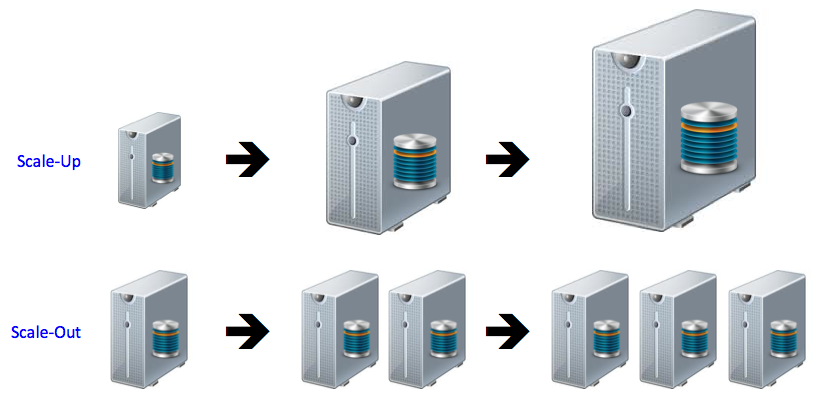
\includegraphics[width=\textwidth]{fig/kb_scale_outup.png}
  \caption{Vertical and horizontal scalability [Source: \cite{ScaleOutPicture}]}
  \label{fig:scale}
\end{figure}

This architecture style enabled another innovation in terms of scaling. As I described in the beginning of this section, with physical servers and also in traditional virtualization, applications are scaled up by adding more processors, memory, or storage. In cloud computing, the application can scale by adding more virtual machines to handle the workload. This approach is called scaling out. This approach is also referred to as horizontal scaling. See the picture \ref{fig:scale} for more details. Such scaling can be also done automatically, on demand. This means that the application does not need to have all the resources reserved for itself all the time. For example, an application can run in business’ private datacentre, which provides the computing power for the majority of time. In a need of extra computing power, the application can automatically scale out and use resources from another datacentre, which might be run by different company as a paid service. This leads us to different models of cloud computing and deployment models.

\subsection{Models of Cloud Computing}
There are several models \cite{CL210} describing the the terms in which are cloud computing resources used. It varies from using the whole infrastructure to using only an environment, in which an application would run.
\begin{itemize}
  \item{\textbf{Infrastructure as a Service (IaaS)} provides computing resources, which can be used to provision virtual machines and software-defined networks. In this model, the cloud consumer manages the application, operating system, storage, networking, and computing resources. OpenStack is an IaaS solution.}
  \item{\textbf{Platform as a Service (PaaS)} provides an operating system including libraries and programming languages. In this model, the cloud consumer manages the application, but not the underlying infrastructure.}
  \item{\textbf{Software as a Service (SaaS)} provides an operating system and the application. In this model, the cloud consumer does not manage the application nor the underlying infrastructure.}
\end{itemize}


\subsection{Models of Cloud Deployment}
There are several ways \cite{CL210} where to deploy the cloud computing infrastructure. A company can a cloud in their own datacentre, or they can use a public provider. A combination of both is also common.
\begin{itemize}
  \item{\textbf{Public cloud} is a cloud run by a cloud provider, provided as a service.}
  \item{\textbf{Private cloud} is a cloud run and used by a single organization.}
  \item{\textbf{Hybrid cloud} is a combination of public and private cloud. The cloud consumer has the ability to run an application in their datacentre and expand to the private cloud when more resources are needed. It is commonly achieved by two independent cloud deployment that use single interface to manage the resources. An example of such interface can be Red Hat CloudForms.}
\end{itemize}


\section{OpenStack}
OpenStack is an open-source cloud platform that controls large pools of compute power, storage, and networking resources of one ore more datacentres. These resources are then used to provision virtual machines.

The service is managed by a single web interface called dashboard or a command-line interface, which gives the administrators control over the whole cloud, and users the ability to provision and manage resources via single web interface.
OpenStack consists of several components. The base six components provide identity, networking, object storage, block storage, a service for managing images, and the compute service. Other services may include an orchestration service, telemetry service to measure usage of the cloud, or a database as a service solution (DBaaS). These services will be described in more detail later in the thesis.

All services communicate with each other via public HTTPS endpoints and use Advanced Message Queuing Protocol (AMQP), which is a protocol supporting sending and receiving messages between distributed systems. \cite{CL210}

\subsection{Core OpenStack Components}
\begin{figure}[!h]
  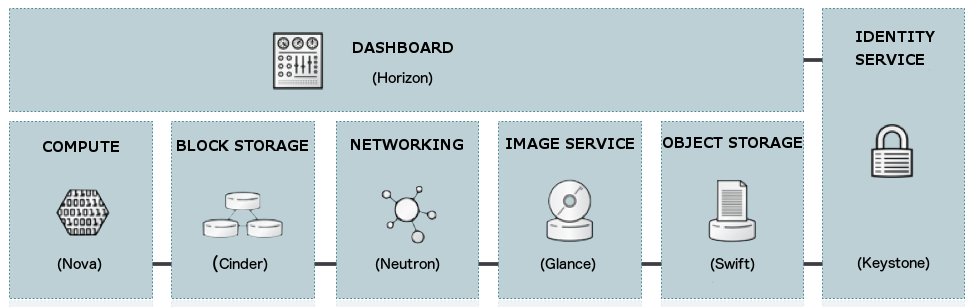
\includegraphics[width=\textwidth]{fig/openstack_services.png}
  \caption{OpenStack core services [Source: \cite{ServicesImageSource}]}
  \label{fig:openstack_services}
\end{figure}
OpenStack is composed of several components \cite{CL210} called services. Some of them can be seen on picture \ref{fig:openstack_services}, and are also described in this section.
\begin{itemize}
  \item{\textbf{Horizon (dashboard)} is a web interface for managing OpenStack services providing graphical user interface. Horizon supports operations like launching instances, managing networking, and setting access controls.}
  \item{\textbf{Keystone (identity)} is a centralized identity service providing authentication and authorization for other services. It also provides a catalogue of services running in the OpenStack cloud.}
  \item{\textbf{Neutron (networking)} provides software-defined networking (SDN) in the OpenStack cloud, including networks, subnets and routers. Other advanced services such as firewalls, virtual private networks (VPN) or quality of service (QoS) are also supported. This service handles the creating and management of the networking infrastructure for the cloud administrator and users.}
  \item{\textbf{Cinder (block storage)} manages persistent block storage volumes used by virtual machines. The service supports creating of snapshots which can be used for backing up data. Then backup can be then used to restore data or to create some new block storage volumes. This service is often used by the virtual machines as a storage.}
  \item{\textbf{Swift (object storage)} provides an object storage that allows users to store and retrieve files. Swift has a distributed architecture that enable horizontal scaling and redundancy. Data replication is managed by software, which allows larger scalability and redundancy than dedicated hardware.}
  \item{\textbf{Glance (image)} is a registry of virtual machine images. Users can copy server images and use them as templates when setting up new virtual servers.}
  \item{\textbf{Nova (compute)} is a service that manages virtual machines running on compute nodes. Nova is designed to scale horizontally on standard hardware and to download images to launch new instances. Nova is a distributed component that interact with Keystone for authentication, Glance for images and Horizon for a web interface. It uses libvirtd, qemu, and kvm for the hypervisor.}
  \item{\textbf{Ceilometer (metering)} is a service that provides a centralized source for metering and monitoring data, which can be used to meter and bill users.}
  \item{\textbf{Heat (orchestration)} an advanced service to orchestrate multiple cloud application using the Amazon Web Services (AWS) template format. The software integrates other core components of OpenStack into a one-file template system. Templates can be used to create most of OpenStack resources, such as instances, floating IPs, volumes, security groups or users. Heat also offers advanced functionality such as high availability, auto scaling and nested stacks.}
\end{itemize}

\section{Ansible}

\subsection{What is Ansible}
Ansible is an automation engine which can be used for application deployment. It is also suitable as a configuration management tool, for orchestration of deployment and provisioning new servers, all of which will be described later in the section. \cite{AnsibleOverview}

\subsubsection*{Deployment}
Application deployment is a process of taking a source code of a software that has been written internally, building it to get the binaries, copying the required files to the servers that are supposed to run the application, and then starting the necessary services.

Tools other than Ansible that can be used for deployment are for example Capistrano, or Fabric, which are both open-source. \cite{UpAndRunning}

As Ansible can manage both deployment and configuration management, using a same tool for these tasks can make it easier and well-arranged for the people using it.

\subsubsection*{Configuration management}
Configuration management typically means writing some kind of description of our servers - a state in which we want the servers to be. This definition of a state can include information about packages that should be installed (or, more precisely, present) on the server, configuration files containing specific values and have specific permission and ownership, that the correct services are running, and so on.

Except Ansible, common configuration management tools are for example Chef, Salt, Puppet, or cfEngine.  \cite{UpAndRunning}

\subsubsection*{Orchestration of deployment}
We need to use orchestration when there are more servers involved and we need to run tasks in a specific order. This can mean, for example, bringing up the database server first and then starting the web servers. Or in case of updating web servers, we need to take them out of the load balancer one at a time to preserve stable service without outages.

Ansible is designed to support orchestration by using a simple model of dependencies build directly into the core architecture - so the tasks are automatically executed in the correct order.

\subsubsection*{Provisioning}
The term provisioning a new server is often used in a cloud environment. It means creating a new virtual machine instance with operating system installed and having the networking and access configured in a way that the machine can be used.

However, provisioning is also used with baremetal machines, because, in the end, all virtual and cloud machines run on a physical server. Ansible can provision all the machines in the datacenter and can be also integrated with several datacentre management tools, like (not limited to) Red Hat Satellite, Hanlon, or Cobler.

Ansible supports several cloud providers including Amazon EC2, Microsoft Azure, Digital Ocean, Google Compute Engine, Linode, Rackspace and clouds supporting the OpenStack APIs. \cite{UpAndRunning}

\subsection{Advantages of the Ansible Technology}
There are several features of the Ansible technology that are important to mention:

\subsubsection{Syntax is Easy to Read}
The ansible configuration management scripts are build on top of YAML syntax, which is a data format language that was designed to be easy to read for people.

When used properly, the ansible playbooks might be seen as an executable documentation. And it will never be outdated, because it is also the code, that gets executed.

\subsubsection*{Push-based mechanism}
There are two main concepts of deploying a change to servers: push-based and pull-based mechanisms.

Some configuration management, that use agents, are pull-based. An example of these tools can be Puppet or Chef. The pull-based mechanism work in the following way:
\begin{enumerate}
  \item{Administrator makes change to the configuration scripts}
  \item{Administrator pushes the changes to a central service}
  \item{Agent running on the server checks for changes periodically}
  \item{Agent downloads the change from the central service}
  \item{Agent executes the configuration script locally and changes the state of the server}
\end{enumerate}
Ansible uses the push-based mechanism, in which the administrator controls when a change is applied to the server. \cite{UpAndRunning} The administrator does not need to wait for a timer to expire before the change is applied. This is an advantage of the Ansible solution, as it offers more control over the overall system. The push-based mechanism works in the following way:
\begin{enumerate}
  \item{Administrator makes change to the configuration scripts}
  \item{Administrator runs the playbook}
  \item{Ansible connects to the servers and executes modules, making changes to the server}
\end{enumerate}
Ansible, however, also supports a pull-based mechanism, using a tool called ansible-pull.

\subsubsection*{No Agents Required}
To manage a server by ansible, it only needs a Python version 2.5 or later and an SSH to be installed. Ansible does not need any agents or additional software to be installed on the servers. It also does not need any special management interfaces, as it runs on the existing network infrastructure using SSH.

\subsubsection*{Thin Layer of Abstraction}
Some configuration management tools provide a thick layer of abstraction, which enables the administrator to manage multiple operation systems using a single script. For example, an abstraction called package could be used to install a package on a system, regardless its type. It could be a yum-based, or a apt-based system. However, these abstractions can be even bigger which means that administrator often need to learn how these abstractions work. Learning these abstractions would be an extra effort, as the administrators should know how their system work anyway.

Ansible does not use these abstractions. This allows the administrator to write scripts for a specific system without the need of learning the abstractions, which makes the learning process shorter, and reading the scripts easier. \cite{UpAndRunning}


\subsection{Ansible Playbooks}
As already mentioned previously, ansible configuration scripts are called playbooks. Playbooks can define the configuration of the target servers, and they can orchestrate the steps in which the configuration is applied. Playbooks consist of several parts: plays, tasks, and modules. \cite{UpAndRunning} \cite{AnsibleDoc}

\begin{figure}[!h]
  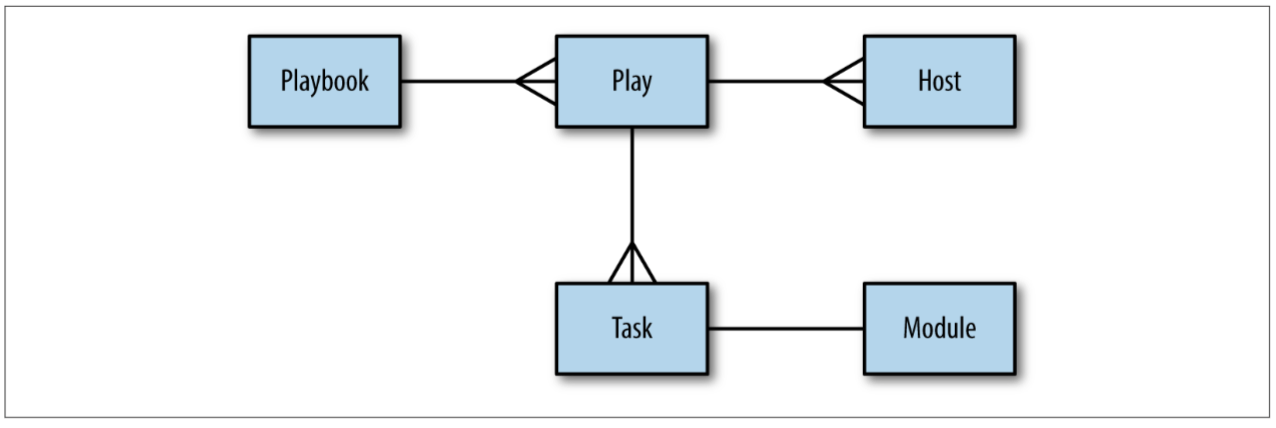
\includegraphics[width=\textwidth]{fig/playbook_anatomy.png}
  \caption{Ansible playbook anatomy [Source: \cite{UpAndRunning}]}
  \label{fig:playbook_anatomy}
\end{figure}

\subsubsection*{Plays}

Playbook is a list of plays. Plays can be thought of as a connection of tasks to hosts. A play must contain:
\begin{itemize}
  \item{A list of hosts}
  \item{A list of tasks that would be executed on the hosts}
\end{itemize}
Plays also support several options that affect the way it is executed. An example of these settings can be:
\begin{itemize}
  \item{\texttt{name} - A description of the respective task. The names should be always used, as they will be printed} at the time of run, showing what changes has been made to a particular server.
  \item{\texttt{sudo} - A boolean value determining if the tasks will be executed with root privileges.}
  \item{\texttt{vars} - A list of variables that would be used for the particular task. They act as a parameters.}
\end{itemize}
An example of a play, taken from \cite{UpAndRunning}, is shown below:

\begin{lstlisting}
- name: Configure webserver with nginx
  hosts: webservers
  sudo: True
  tasks:
    - name: install nginx
      apt: name=nginx update_cache=yes

    - name: copy nginx config file
      copy: >
        src=files/nginx.conf
        dest=/etc/nginx/sites-available/default

    - name: enable configuration
      file: >
        dest=/etc/nginx/sites-enabled/default
        src=/etc/nginx/sites-available/default
        state=link

    - name: copy index.html
      template: >
        src=templates/index.html.j2
        dest=/usr/share/nginx/html/index.html mode=0644

    - name: restart nginx
      service: name=nginx state=restarted
\end{lstlisting}



\subsubsection*{Tasks}

Play is a list of tasks. Every task represents a single module that would be executed. Every task must contain:
\begin{itemize}
  \item{A name of the particular module}
  \item{A list of arguments for the module}
\end{itemize}

Task can also include a definition of its name. Using of names is a good practise, as they are printed at the time of run and can be used to track changes made by the scripts. They also act as comments, improving readability of the playbook.

\subsubsection*{Modules}

Modules are scripts that perform the desired action on the target server.

They are designed to be \emph{idempotent}, which means that they can be run multiple times, but will only make changes when there is a difference between the present and desired state. In other words, running a playbook for the second time without making changes will not affect the target server in any way.

An example of modules can be:
\begin{itemize}
  \item{\texttt{copy} - Copies a file from the local machine to the remote host.}
  \item{\texttt{service} - Manages the services running on the remote host. It can start, stop, or restart a services.}
\end{itemize}


\subsubsection*{Handlers}

When ansible execute modules on a particular server, they may or may not make a change. They only make change when the present state is different from the desired state. At the time of run, ansible prints out the names of tasks that are being executed. If the state has changed, the module will return changed state. And if no action was needed, an ok state will be returned instead. Ansible will then print the result, as seen on the following example:

\begin{lstlisting}
TASK: [Install packages] **********************************
changed: [webserver1]

TASK: [Set configuration] *********************************
ok: [webserver1]
\end{lstlisting}

This detection of a change can be used by a mechanism called handlers. \cite{UpAndRunning} Handlers are actions triggered at the end of run only when a specific change has occurred. However, the action will be executed only once.

For example, a change of a web server configuration might require restart of the particular service. Also, an update of the web server package might require a restart of the service. If any of these actions occur, a handler responsible for restarting the service will be notified and executed at the end of run. It will be executed only once, even when both of the changes above will occur.

\subsubsection*{Roles}

Roles are the main mechanism to break large playbooks into multiple files, which simplifies writing complex playbooks. It also makes them easier to reuse.

When managing a large number of servers, a single playbook describing changes of all of the servers would become too long and hard to maintain. Also, applying a common configuration to multiple servers would result in a duplication of code. To solve this problem, a mechanism called Roles has been introduced to Ansible. \cite{AnsibleDoc}

A role can be thought of as something that should be assigned to one or more hosts. For example, a database role will be assigned to servers acting as a database servers.

Roles can also be dependent, which means that a role can require other role to be applied before. Using this feature, Ansible will automatically ensure that roles are applied in the correct order.
 % viz. obsah.tex
\chapter{OpenStack Architecture}
\label{ch:arch}
This chapter describes the OpenStack architecture, how the components communicate and what they are used for. Selected components, which are needed for the deployment option used later in this thesis, will be described in more detail.

\section{Conceptual Architecture}
Conceptual architecture is a high level architecture that shows the core components of a system and their relations including description of responsibilities for each component.

The relationships among the OpenStack services can be seen on picture \ref{fig:OpenStack_conceptual_arch}.
\begin{figure}[!h]
  \includegraphics[width=\textwidth]{fig/OpenStack_conceptual_arch.png}
  \caption{OpenStack conceptual architecture [Source: \cite{conceptualArch}]}
  \label{fig:OpenStack_conceptual_arch}
\end{figure}





\section{Logical Architecture}
Logical architecture shows processes and functions that make the system functioning.

OpenStack consists of several independent parts called OpenStack services.\cite{CL210} Authentication for all services is provided by a common identity service. The services interact with each other via public APIs. \cite{AdminGuide}

OpenStack services are internally composed of several processes. Each service has at least one API process. This API process listens for API requests, does necessary preprocessing and passes them to the particular process or processes within the service. The actual work of a service is done by distinct processes. An exception to this rule is the identity service.

The processes within a service communicate with each other via message broker using AMQP protocol. The most used AMQP broker is RabbitMQ, which is also used in this thesis.

The state of a service is stored in a database. OpenStack support several databases, such as MySQL, MariaDB, and SQLite. The database solution used in this thesis is MariaDB. \cite{AdminGuide}

Users can interact with OpenStack in several ways. There is a graphical web-based interface, which is implemented by OpenStack Dashboard. Other ways include command-line clients provided by all basic services, and by API requests using web browser plugins or curl.

The most common, but not the only possible logical architecture can be seen on picture \ref{fig:OpenStack_logical_arch}.

\begin{figure}[!h]
  \includegraphics[width=\textwidth]{fig/OpenStack_logical_architecture.png}
  \caption{OpenStack logical architecture [Source: \cite{logicalArch}]}
  \label{fig:OpenStack_logical_arch}
\end{figure}

\section{Physical Architecture}
OpenStack is a distributed system, which enables cloud architects to design varieties of physical architecture reflecting needs of the cloud consumer.

\textit{“Designing an OpenStack cloud is a great achievement. It requires a robust understanding of the requirements and needs of the cloud’s users to determine the best possible configuration to meet them. OpenStack provides a great deal of flexibility to achieve your needs...”} \cite{OperationsGuide}




\section{Installation of Core Components}

This section will explain each service of the OpenStack cloud in more detail including general description, some basic principles of the function, and a list of components of the service. Some services, such as Compute or Storage, can use several backends for the actual work. List and short description of these backends is also included in this section.


\subsection{OpenStack Identity Service}
The OpenStack identity service provides a single point of authentication and authorisation. When OpenStack services receive a request from a user, they check with the identity service to verify the authorisation of the user.

It also provides a catalog of OpenStack services. When installing OpenStack cloud, each service needs to be registered in the identity service. The identity service then tracks which services are installed and where they are located on the network.

OpenStack services also use the identity service as a common unified API.

\subsubsection*{Identity Abstractions}

The identity service uses the following abstractions:
\begin{itemize}
  \item{\textbf{Service} is an OpenStack service, such as the identity (Keystone) service, compute (Nova) service, etc.}
  \item{\textbf{Endpoint} is an address accessible via network and acts as an access-point of a service.}
  \item{\textbf{Region} represents a general division of the OpenStack deployment. The identity service also supports sub-regions, which allows the creation of a tree-structured hierarchy.}
  \item{\textbf{Authentication} is the process of confirming the identity of a user. To confirm an incoming authentication request, the identity service validates a set of credentials supplied by the user. These can be a name and password, or a name and API key. After validation of the user credentials, the identity services then issues an authentication token. This process is done only once on in the beginning of a session and user then provide this token in all subsequent requests.}
  \item{\textbf{Credentials} are data to identify the user, such as name and password, or name and API key.}
  \item{Authentication \textbf{token} is an alpha-numeric string used to access to OpenStack APIs and resources. Token is valid for a finite duration and can be revoked at any time.}
  \item{\textbf{Domain} is a collection of projects and users. This collection defines administrative boundaries for managing identity entities. Domains can be used to represent an individual person, a company, or an operator-owned space. User can be granted the administrator role within a domain. This domain administrator can then create users, projects, and groups in the domains as well as create and assign roles to users or groups.}
  \item{\textbf{Project} is used to isolate resources or identity objects. Projects can be used to map to a customer, account, organisation, or tenant.}
  \item{\textbf{Role} is a personality containing a set of user rights and privileges. A user contains a list of roles.}
  \item{\textbf{Group} is a collection of users and is owned by a domain. A group can be assigned a role that applies to all users in the group.}
  \item{\textbf{User} is a representation of a person, system or service using the OpenStack services.}
  \\\cite{CL210}
\end{itemize}


\subsubsection*{OpenStack Identity Components}

The identity service consists of these components:
\begin{itemize}
  \item{\textbf{Server} - A centralised server, providing authentication and authorisation services. It uses a RESTful interface.}
  \item{\textbf{Drivers} - Drivers are used to access identity information provided by external repositories like LDAP, or existing SQL databases.}
  \item{\textbf{Modules} - Middleware modules that check service requests, extract user credentials and send them to the Server for authorisation. The modules are integrated with the OpenStack components by using the Python Web Server Gateway Interface (Python WSGI).}
 \\\cite{InstallGuide}
\end{itemize}


\subsection{OpenStack Image Service}
The OpenStack Image service controls image storage and management and allows users to discover, register, and retrieve images.

Images provide templates for virtual machine filesystems. Each virtual machine runs from a copy of a base image and several virtual machines can be run from a single base image. Any changes made to the virtual machines will not affect the image. Users can also create a snapshot - a state of a virtual machines running disk - and build a new image based on these snapshots.

The implementation of the image service is called Glance. It supports various backends as a storage, which can be normal filesystems, OpenStack object storage, HTTP, RADOS block devices, and Amazon S3. Some of the storage backends can be read-only. The architecture in this thesis will use normal filesystem mounted to the controller node.

\subsubsection*{Basic Components}
The image service consists of the following components:
\begin{itemize}
  \item{\textbf{glance-api} - Accepts API calls.}
  \item{\textbf{glance-registry} - Stores, processes, and retrieves metadata about images like size and type. This is an internal service only and should not be exposed outside of the image service.}
  \item{\textbf{Database} - An SQL database to store image metadata.}
  \item{\textbf{Storage} repository for image files - Backend that stores the images itself.}
\end{itemize}





\subsection{OpenStack Compute Service}
The OpenStack Compute service is the major part of an Infrastructure as a Service (IaaS) system. It runs and manages the virtual machines running in the OpenStack cloud. It can also provide networking for the virtual machines. However, Nova networking is not often used. The OpenStack Networking (Neutron) , described in this section, is used instead. \cite{InstallGuide}

The OpenStack Compute service scales horizontally and is commonly deployed on multiple hosts, \cite{OperationsGuide} often called compute nodes.

The service manages virtualisation, but it does not include any virtualisation software. Instead, it uses drivers to interact with the underlying virtualisation backend, also called virtualisation provider. It is also possible to use multiple providers in different availability zones.

The OpenStack Compute service supports these following virtualisation providers: \cite{AdminGuide}
\begin{itemize}
  \item{Baremetal}
  \item{Docker}
  \item{Hyper-V}
  \item{Kernel-based Virtual Machine (KVM)}
  \item{Linux Containers (LXC)}
  \item{Quick Emulator (QEMU)}
  \item{User Mode Linux (UML)}
  \item{VMware vSphere}
  \item{Xen}
\end{itemize}

\subsubsection*{Service Architecture}

The architecture of the Compute service could be divided into the following four parts:
\begin{itemize}
  \item{\textbf{API Server} is the compute controller that commands and controls the hypervisor, storage, and networking available to the end users. It manages the API endpoints, which are basic HTTP web services that handle the authentication, authorisation, and basic command and control functions. It support various API interfaces including Amazon, Rackspace, and others, which enables compatibility with multiple existing tools already created for other cloud platforms. This open approach also prevents vendor lock-in.}
  \item{\textbf{Message Queue} manages the interaction between compute nodes, the networking controllers, API server, and the scheduler. It is provided by the Advanced Message Queuing Protocol (AMQP). Several implementations are available, the most common are RabbitMQ, Qpid, ZeroMQ, and others.}
  \item{\textbf{Compute Worker} manages the virtual machines that run on the compute nodes. It is managed via API that provides commands to run, delete, and reboot instances, attaching and detaching volumes, and to get local console output.}
  \item{\textbf{Network Controller} manages the networking resources available on the compute nodes. It is managed via API that provides commands for allocating fixed IP addresses, configuring VLANs for projects, or configuring networks for compute nodes.}
  \\\cite{AdminGuide}
\end{itemize}

\subsubsection*{OpenStack Compute Components}

The OpenStack Compute service consists of the following components:
\begin{itemize}
  \item{\textbf{\texttt{nova-api} service} - Accepts API calls and responds to them. It supports the OpenStack Compute API, the Amazon EC2 API, and a special Admin API.}
  \item{\textbf{\texttt{nova-api}-metadata service} - Accepts metadata requests from instances.}
  \item{\textbf{\texttt{nova-compute} service} - A worker daemon that manages virtual machines via virtualisation provider API. It supports XenAPI, libvirt, VMwareAPI, and others. The state of the instances is always saved in the database.}
  \item{\textbf{\texttt{nova-scheduler} service} - This service determines on which compute node a new virtual machine should be started.}
  \item{\textbf{\texttt{nova-conductor} module} - It is a point of access to the database for other nova services. It eliminates direct access to the database by other services. This service scales horizontally and can be deployed on multiple hosts.}
  \item{\textbf{\texttt{nova-cert} module} - This is only needed to use with the Amazon EC2 API, used to generate certificates.}
  \item{\textbf{\texttt{nova-network} worker daemon} - Similar to the nova-compute service, but for networking. Accepts networking tasks from the queue and manipulates the network.}
  \item{\textbf{\texttt{nova-consoleauth} daemon} - Provides authorisation for users provided by the console proxies - see nova-novncproxy and nova-xvpvncproxy for more information. It needs to run for the proxies to work.}
  \item{\textbf{\texttt{nova-novncproxy} daemon} - Proxy for accessing running virtual machines via a VNC connection. Supports browser-based HTML5 clients.}
  \item{\textbf{\texttt{nova-spicehtml5proxy} daemon} - Proxy for accessing running virtual machines via a SPICE connection. Supports browser-based HTML5 clients.}
  \item{\textbf{\texttt{nova-xvpvncproxy} daemon} - Proxy for accessing running virtual machines via a VNC connection. Supports an OpenStack-specific Java client.}
  \item{\textbf{\texttt{nova-cert} daemon} - Manages x509 certificates.}
  \item{\textbf{\texttt{euca2ools} client} - A set of command-line interpreter commands to manage the cloud resources via Amazon EC2 interface.}
  \item{\textbf{\texttt{nova} client} - A command-line client for the end user.}
  \item{\textbf{Message Queue} - Passes messages between nova daemons. Provided by the Advanced Message Queuing Protocol (AMQP). It is usually implemented by RabbitMQ.}
  \item{\textbf{SQL Database} - Stores most of the build-time and run-time states of the infrastructure, including information about available virtual machine types, virtual machines in use, available networks, and information about projects. OpenStack Compute supports SQLite3 for test and development work, MySQL and MariaDB, and PostgreSQL.}
  \\\cite{InstallGuide}
\end{itemize}



\subsection{OpenStack Networking Service}
The OpenStack Networking service enables users to create virtual networks and attach the devices managed by other OpenStack services to them. It provides an API that lets users to configure and manage network connectivity and addressing. The network services include L3 forwarding, NAT, load balancing, firewalls, and VPN.

Networking provides the end users the ability to create virtual networks, subnets, routers, and firewalls. All of these will be explained later in this section.

It also supports variety of plug-ins which can enable interoperability with several commercial and open source technologies. This plug-in architecture provides flexibility when designing custom OpenStack architecture and deploying it.

\subsubsection*{Networking}
Before using or deploying the OpenStack Networking service, the following general facts about networking \cite{NetworkingGuide} should be understood:

\begin{itemize}
  \item{\textbf{Ethernet} is a networking protocol that is being used by most wired network interface cards. In the OSI model of networking, Ethernet operates on the second layer, also referred to as layer 2, L2, link layer, or data link layer. Every host has unique identification called Media Access Control (MAC) address.

  Ethernet can be conceptually think of as a single bus, to which each of the network host is connected. However, modern networks use devices called switches, and every device is connected directly to them.

  The OpenStack Dashboard uses this simple model to visualise the network topology to the end user. This ethernet network is sometimes referred to as a layer 2 segment.}
  \item{\textbf{VLAN} is a networking technology that creates separate virtual network on a single switch in a way, that devices connected to the same switch can not each other's traffic, if they are on different VLANs.

  OpenStack uses VLANs to isolate the traffic of different tenants, even when their instances run on a single host.

  Each VLAN has a numerical ID between 1 and 4095. For example, a VLAN with an id of 15 will be referred to as VLAN 15.}
  \item{\textbf{Address Resolution Protocol (ARP)} - As pointed out above, network devices use MAC addresses to be identified. However, TCP/IP applications use IP addresses as an identifiers. The Address Resolution Protocol (ARP) bridges the gap by translating IP addresses into MAC addresses.}
  \item{\textbf{Dynamic Host Configuration Protocol (DHCP)} dynamically assigns IP addresses to network hosts. These hosts are called DHCP clients.}
  \item{\textbf{TCP, UDP, and ICMP} - Software applications communicating over an IP network use another protocols above IP. In the OSI model of networking, they use the fourth layer, which is also referred to as layer 4, or transport layer. There are three main protocols:
    \begin{itemize}
      \item{\textit{Transmission Control Protocol (TCP)} is the most commonly used layer 4 protocol. It is a connection-oriented protocol. Delivery of packets via this protocol is guaranteed.}
      \item{\textit{User Datagram Protocol (UDP)} is mostly used to transfer real-time information like voice or video. It is a connectionless and unreliable protocol which means that the delivery of packaets via this protocol is not guaranteed.}
      \item{\textit{Control Message Protocol (ICMP)} is used for sending control messages.}
    \end{itemize}
  }
  \item{\textbf{Switch} is device that allow packets to travel from one node to another. They connect hosts belonging to the same layer-2 network. Switches forward the traffic based on the destination Ethernet address in the packet header.}
  \item{\textbf{Router} is device that allows communication between nodes on different layer-3 networks. They route the traffic based on the destination IP address in the packet header.}
  \item{\textbf{Firewall} is device that restricts traffic to and from hosts on a network by special rules defined on the device. They are supposed to protect hosts from unauthorised access and attacks.}
  \item{\textbf{Load Balancer} is device that allows even distribution of traffic across several hosts. They are supposed to avoid overload of a single host. They also prevent a single point of failure as they enable the traffic to be processed by multiple hosts.}

\subsubsection*{Networking Concepts in OpenStack}
OpenStack uses the following concepts to enable users to create their own virtual network infrastructure:
  \item{\textbf{Network} is an isolated L2 segment. There are two types of network:
    \begin{itemize}

      \item{\textit{Tenant Networks} are managed by the end user and are used within their projects. These networks are fully isolated from other projects.}
      \item{\textit{Provider Networks} are managed by the OpenStack administrator and map ti the existing physical network in the datacenter. These networks are mainly used to enable external connectivity to the virtual machines running in the cloud. Each project should have at least one public provider network.}
    \end{itemize}
    }
  \item{\textbf{Subnet} is a block of IP addresses and associated configuration state. They are used to allocate IP addresses to ports that are created on a network.}
  \item{\textbf{Port} - Not to be confused with TCP or UDP port. In the OpenStack terminology, port is a connection point for attaching a single device (such as NIC of a virtual machine) to a virtual network. It also describes the configuration like MAC address and IP address.}
  \item{\textbf{Security Groups} enable users to define their own firewall rules in groups. They can control traffic in both direction (called ingress and egress). These rules are then applied to a port. A port can be assigned with multiple security groups.}
  \\\cite{NetworkingGuide}
\end{itemize}

\subsubsection*{OpenStack Networking Components}
The OpenStack Networking service is composed of the following components \cite{InstallGuide}:
\begin{itemize}
  \item{\textbf{neutron-server} - accepts API requests and routes them to the appropriate Networking plug-in}
  \item{\textbf{OpenStack Networking plug-ins and agents} - the main logic is implemented by several plug-ins. They plug and unplug ports, create networks, subnets, and provide IP addressing. OpenStack Networking ships with plug-ins and agents for Cisco virtual and physical switches, NEC OpenFlow products, Open vSwitch, Linux bridging, and the VMware NSX product. The architecture in this thesis will use Linux bridging.}
  \item{\textbf{Messaging queue} - routes the information between neutron-server and other agents. It also act as a database for particular plug-ins. The architecture in this thesis will use centralised RabbitMQ service running on a controller node.}
\end{itemize}

The architecture in this thesis will use the following plug-ins and agents for networking:
\begin{itemize}
  \item{\textbf{Modular Layer 2 plug-in} - builds layer-2 (bridging and switching) virtual networking infrastructure for virtual machines. IT uses the Linux bridge mechanism.}
  \item{\textbf{Linux bridge agent} - builds the networking infrastructure for virtual machines and also manages VXLAN tunnels for private networks and security groups.}
  \item{\textbf{Layer 3 agent} - is the most commonly used agent that provides layer-3 (routing) services for virtual networks.}
  \item{\textbf{DHCP agent} - provides DHCP services for virtual networks.}
\end{itemize}







\subsection{OpenStack Block Storage Service}
The OpenStack Block Storage service adds persistent block storage to a virtual machine instances and provides an infrastructure for managing volumes. This service is similar to the Amazon EC2 Elastic Block Storage (EBS) offering.

The service supports various backends which can be consumed using a Block Storage driver. An example of supported drivers that are available can be NAS/SAN, NFS, iSCSI, Ceph, and more. A usage of multi-backend configuration is also supported. \cite{InstallGuide}

To install the OpenStack Block storage service, it is important to understand a number of concepts, because there are several choices of deployment. \cite{OperationsGuide} Apart from choosing the right storage backend, it mostly depends on the final architecture - which can be single node or multi-node. For example, in this thesis I use a multi-node architecture with separate block storage node, and will use a local LVM storage as a backend.

\subsubsection*{Logical Volume Management (LVM)}
Because this thesis will use an LVM as a block storage provider, it is important to understand the basic concepts of LVM.

LVM creates a layer of abstraction over physical storage, which allows you to create multiple logical storage volumes. From an application view, these logical volumes are the same as traditional disk partitions. The hardware storage configuration is also hidden from the software, so it can be resized and moved without stopping services or unmounting filesystems. And in an opposite way, the logical volumes can be also resized without changing the underlying physical storage. This solution provides much more flexibility than using traditional partitions directly. \cite{LVMPdf}

\begin{figure}[!h]
  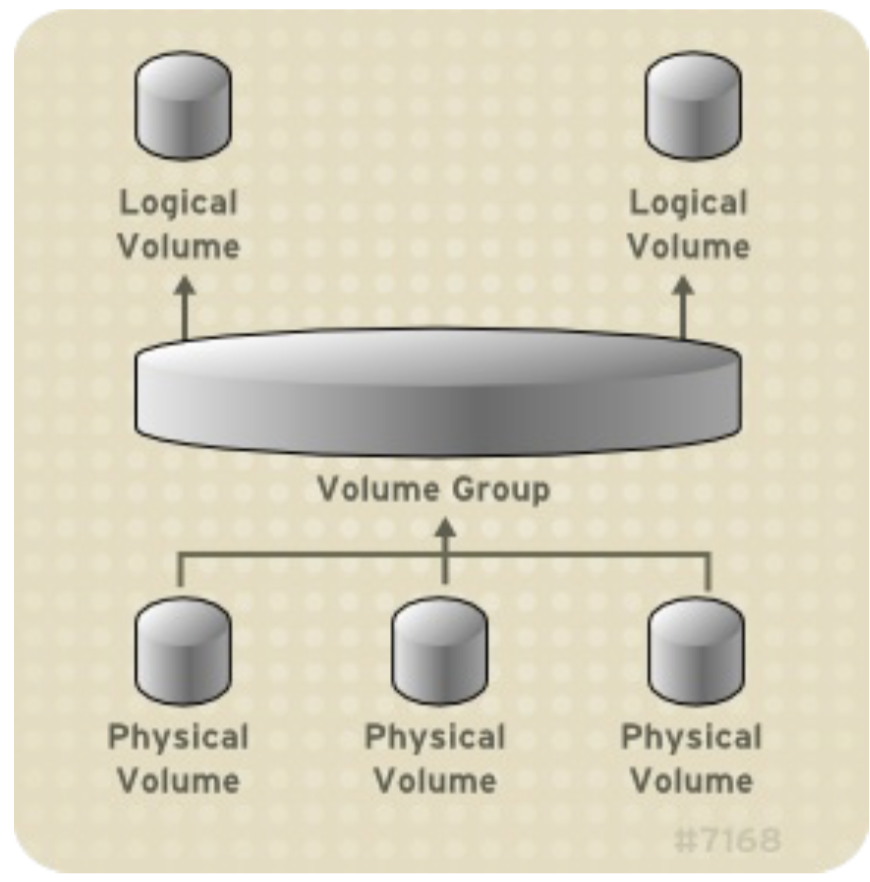
\includegraphics[width=\textwidth]{fig/lvm_architecture.png}
  \caption{Logical volume architecture [Source: \cite{lvmArch}]}
  \label{fig:lvm_architecture}
\end{figure}

As shown on the picture \ref{fig:lvm_architecture}, LVM consists of three basic layers:
\begin{itemize}
\item{\textbf{Physical Volume (PV)} is the underlying physical block storage device, which can be a partition or the whole disk. To use the device for LVM, it needs to be initialised as a Physical Volume (PV).}
\item{\textbf{Volume Group (VG)} is a combination of several physical volumes. However, volume group can also consist of a single physical volume. This layer provides a pool of disk space used to create logical volumes (LV) in the same way disks are divided into partitions.}
\item{\textbf{Logical Volume (LV)} is the volume used by filesystems and applications. In LVM, a volume group is divided into several logical volumes.}
\end{itemize}

\subsubsection*{Block Storage Components}

The OpenStack Block Storage service consists of the following components \cite{InstallGuide}:
\begin{itemize}
\item{\textbf{cinder-api} - Accepts API requests and routes them to the cinder-volume process for action.}
\item{\textbf{cinder-volume} - This process manages the read and write requests sent to the Block Storage service. It interacts with the cinder-scheduler and cinder-backup processes and the storage providers, using respective drivers.}
\item{\textbf{cinder-scheduler daemon} - In multi-node deployments, it selects the optimal storage node on which the volume will be created. This process is similar to the nova-scheduler.}
\item{\textbf{cinder-backup daemon} - Provides the ability to back up volumes. It can interact with multiple backup storage providers using drivers, in a similar way as the cinder-volume process.}
\item{\textbf{Messaging queue} - Routes information between the processes within the OpenStack Block Storage service. In this thesis, I use a centralised RabbitMQ service, running on the controller node.}
\end{itemize}




\subsection{OpenStack Dashboard Service}
The OpenStack Dashboard service provides you a way to manage the OpenStack resources and services. It is used by administrators and the end user. It provides a web-based interface that communicates through the OpenStack APIs. It also allows customising the brand of the dashboard to match the cloud provider's needs. \cite{InstallGuide}

\subsubsection*{Handling of User Session Data}

The Dashboard service supports several session backends \cite{DeployingHorizon} to handle the user session data:
\begin{itemize}
  \item{\textbf{Local Memory Cache} - The quickest and easiest session backend, which does not require external dependencies and is the easiest to set up. However, it does not support shared storage across processes or workers, and does not offer data persistency after a process terminates. This is the reason why it is not recommended for production use.}
  \item{\textbf{Memcached} - An external caching service. Supports shared storage and offers data persistency after process or worker terminates. It is extremely fast and efficient cache backend. It requires the memcached service to be running and accessible and a python memcached module installed.}
  \item{\textbf{Database} - A database can be also used as a caching backend. It is scalable, it can be highly-available and offers data persistency. However, it is slow in comparison to other caching methods.}
  \item{\textbf{Cached Database} - This is a hybrid setting using database and caching infrastructure together.}
  \item{\textbf{Cookies} - Stores data in a cookie in the user's browser. It supports a cryptographic signing to ensure that the data has not been changed during transport. It should be noted, that signing is not the same as encryption, so that the data are still readable by potential attacker.}
\end{itemize}

In this thesis, I will use the Memcached option.

\chapter{Existing Methods of Automated OpenStack Deployment}
\label{ch:existing}
\section{Packstack}
Packstack is a command line installation utility that support deployment of OpenStack on existing server using SSH connection. The installation can be configured interactively or by a configuration file called answer file. \cite{CL210}

It is suitable for deploying proof-of-concept installations. It supports these two basic types of deployment:
\begin{itemize}
  \item{\textbf{An all-on-one installation} - All services are installed on a single physical host that would run all controller services and the virtual machines.}
  \item{\textbf{Multiple nodes} - Using several hosts to run the installations, where there is a single controller node running the controller services, and one or more compute nodes that would run the virtual machines.}
  \\\cite{PackstackRDO}
\end{itemize}

However, packstack is not suitable for production deployments. This is mainly because it makes many assumptions in the configuration in order to simplify the installation process. It can not deploy the services in a high availability (HA) mode or using load balancers. It also does not support advanced networking configuration, which might be required by more complex setups. \cite{PackstackRedHat}

\section{OpenStack-Ansible}
OpenStack-Ansible is an official OpenStack project, still under development. The goal of this project is to be able to deploy OpenStack cloud in a production environment directly from source code. It is focused on Ubuntu Linux and the OpenStack components are installed into Linux Containers (LXC). \cite{OpenStackAnsibleOfficial} \cite{OpenStackAnsibleOfficialGit}

\chapter{Implementation Design}
\label{ch:implementation}

\section{Design of the Physical Architecture}
\label{sec:phys}

\subsection{Selecting OpenStack Services}
The first decision when designing an OpenStack cloud deployment is about the services we need to have running.

For this thesis, I have chosen these five core services:
\begin{itemize}
  \item{OpenStack Identity (Keystone)}
  \item{OpenStack Image (Glance)}
  \item{OpenStack Compute (Nova)}
  \item{OpenStack Block Storage (Cinder)}
  \item{OpenStack Dashboard (Horizon)}
\end{itemize}

These services will be also required:
\begin{itemize}
  \item{SQL Database}
  \item{AMQP message broker}
\end{itemize}



\subsection{Selecting Specific Implementations}
The second decision is about technology. The most important is to choose a specific version of OpenStack. The OpenStack release chosen for this thesis will be Liberty. This is mostly because it is the  latest release at the time of writing the thesis.

I also need to choose an operating system platform that will run on the physical host machines. Choosing the right Linux distribution is important as there might be big differences in terms of available packages, stability, the lifecycle, and an option of commercial support. The target platform of deployment will be CentOS 7.2. CentOS is free and open source operating system based on the Red Hat Enterprise Linux platform. It uses the RPM packaging model and the OpenStack Liberty packages are included in the repositories. The system is stable, has a long lifecycle and potential migration to to a commercially supported environment would be easy, as it is based on the Red Hat Enterprise Linux platform.

OpenStack also needs an SQL database to store the state of the services, and it also might me used as a storage for the Identity service. In this deployment, it will be used in this way. I have chosen MariaDB because it is open source, widely used and handles memory well.

The next component is an AMQP broker. It is used by processes within the OpenStack service for communication, and it also might be used as a short-term storage by some networking plugins. For this particular deployment, I will use RabbitMQ because it is an open source solution and it is widely used in production environments. It is also well-supported by the OpenStack itself.

The last decision will be about storage backend for the OpenStack Block Storage service. I will use a local disk and an LVM technology. LVM is a robust and stable open source solution for storage that runs on commodity hardware, which is important especially for this testing environment.


\subsection{Physical architecture}

\begin{figure}[!h]
  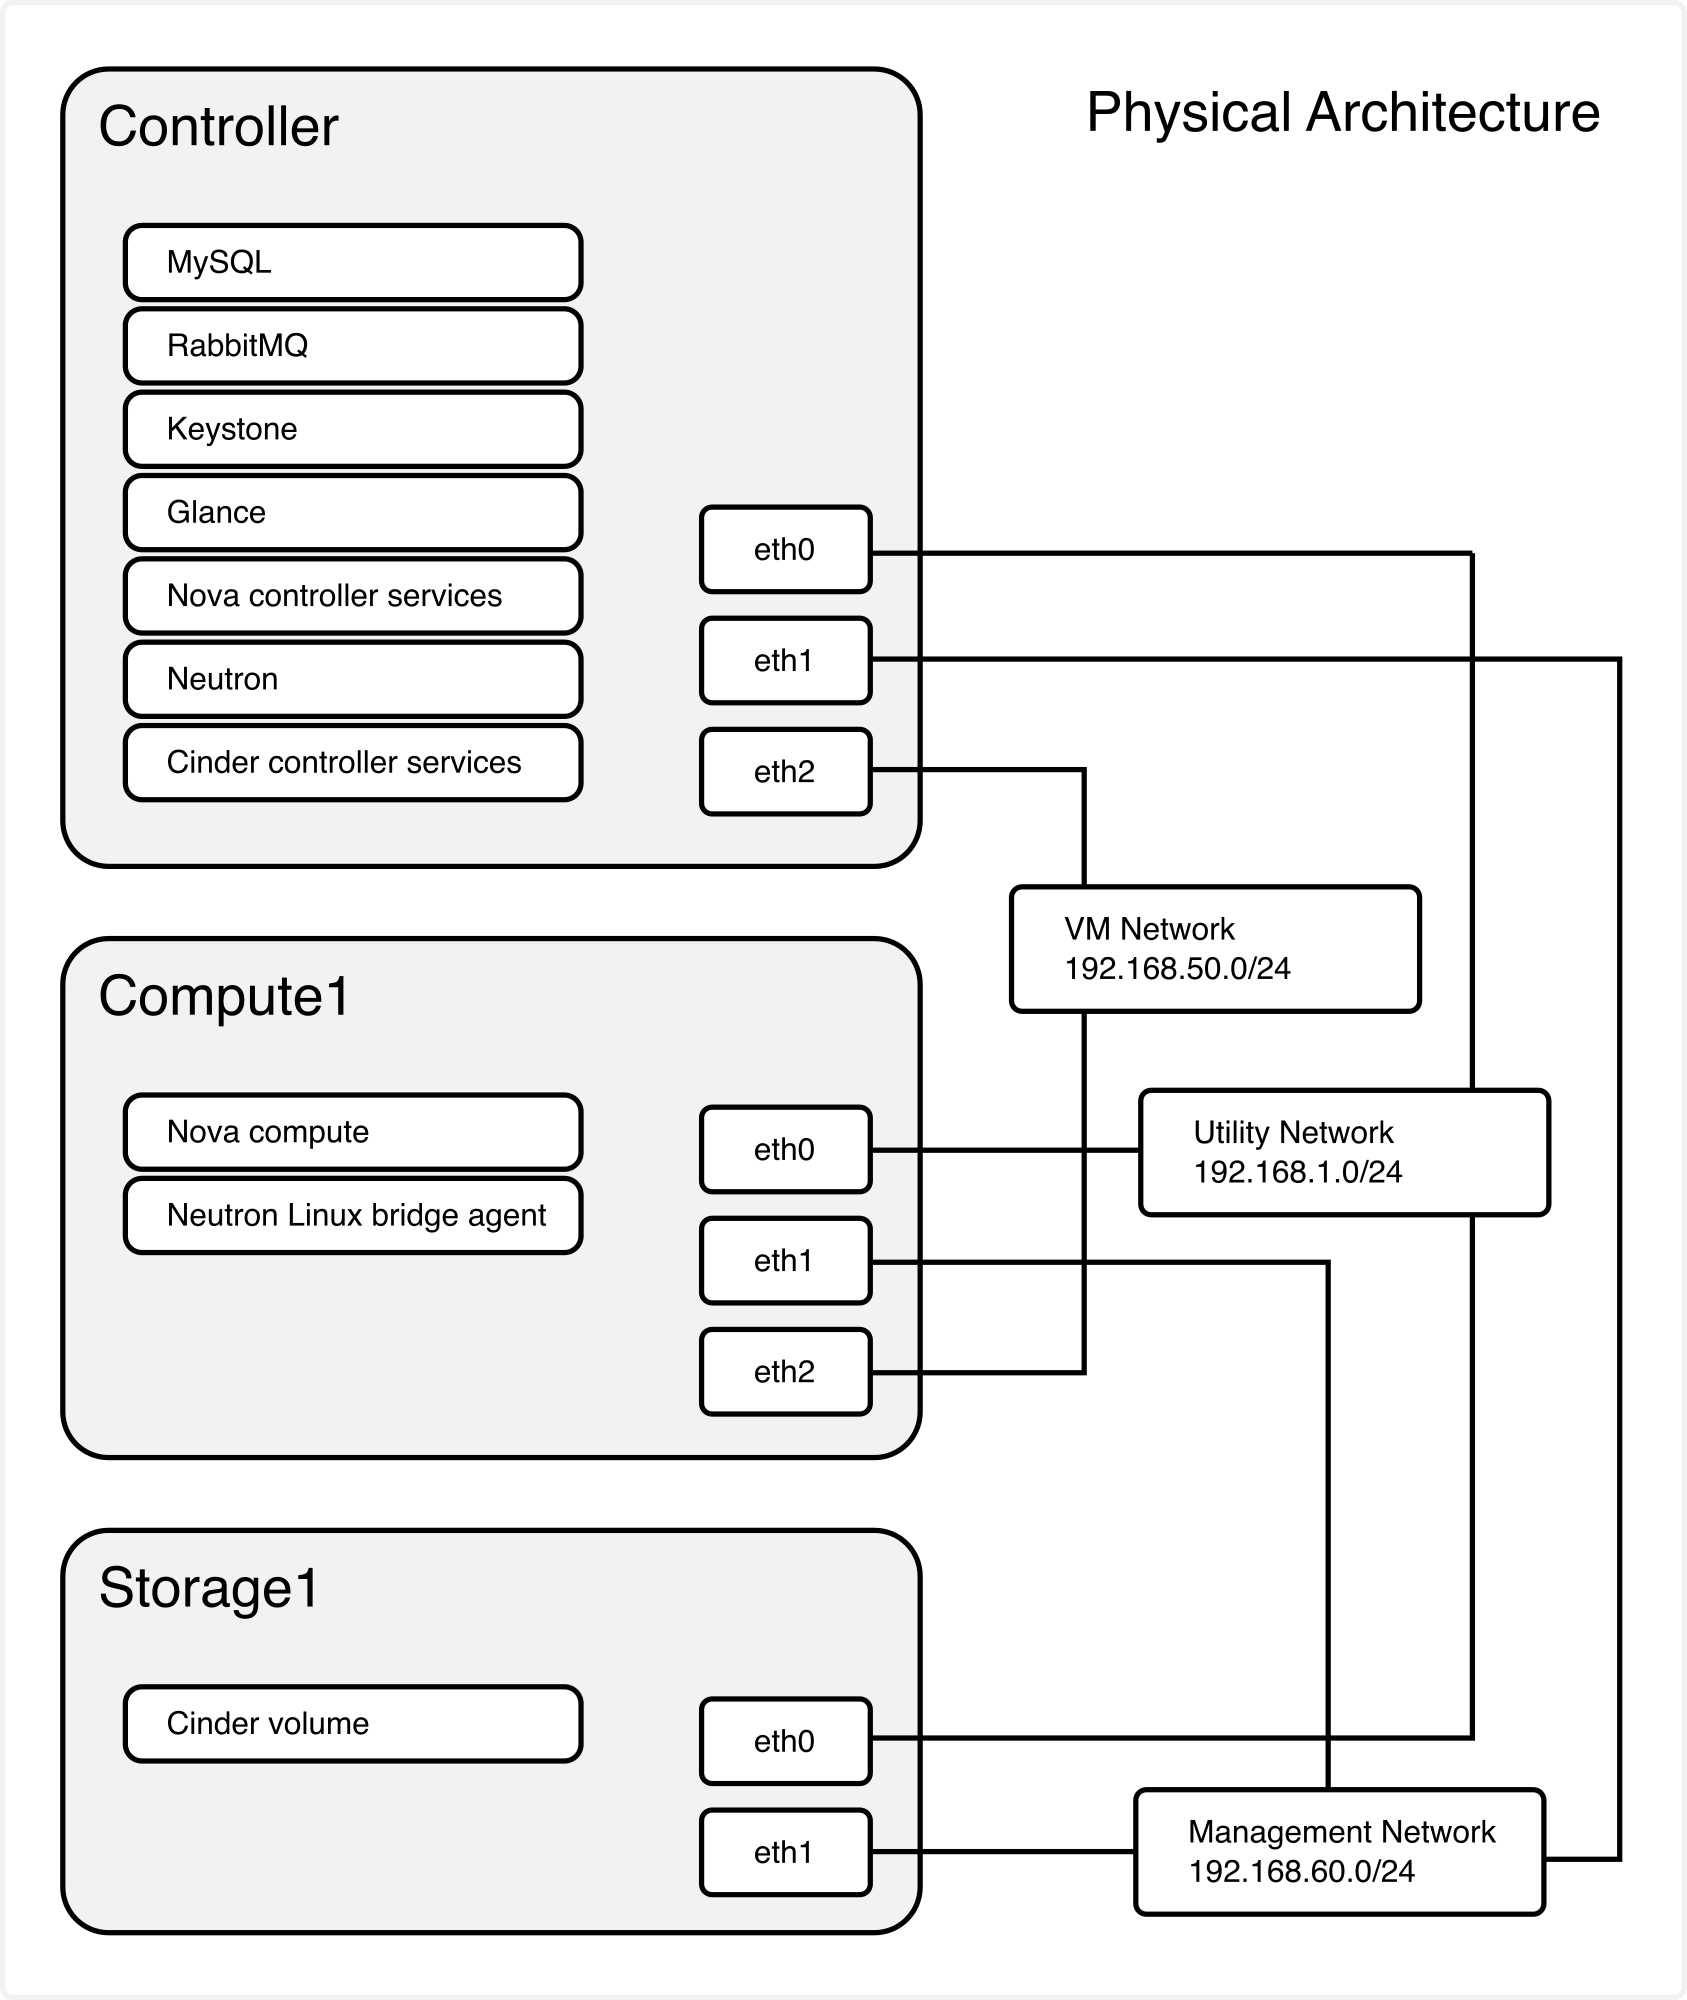
\includegraphics[width=\textwidth]{fig/my_architecture.png}
  \caption{OpenStack physical architecture design}
  \label{fig:openstack_physical_arch}
\end{figure}

\subsubsection*{Networks}
I have used three different networks in my architecture and each one have different purpose in the whole system. Their descriptions are as follows:
\begin{itemize}
  \item{\textbf{Utility Network} - This network is used the datacenter administrators to maintain the physical hosts. In this example it will also be used by Ansible to deploy the OpenStack and all other services.}
  \item{\textbf{Management Network} - This network is used by the OpenStack services to communicate with each other. It will also provide connectivity for the services to the MySQL database and the RabbitMQ Message Queue. All Keystone endpoints based on hostnames will also use this network. It will be also used to connect storage from Storage1 host to virtual machines running on the Compute1 host.}
  \item{\textbf{VM Network} - This network is used to provide outside connectivity to the virtual machines running on the compute node.}
\end{itemize}
It is also important to note that the eth2 interfaces on Controller and Compute1 hosts will use special configuration without an IP address and will be attached to virtual network bridges. Their specific configuration will be mentioned later in the text.



\section{Design of the Ansible Playbook}
\subsection{Ansible Roles}
The services will be installed on the target hosts using Ansible roles. Roles offer flexibility in a way, that each role can be installed separately on a given host, or, if needed, on multiple hosts. These roles can be then reused to deploy a different physical architectures.

All roles use handlers to restart services in case of a configuration change. All roles are also designed to be idempotent.

\subsubsection*{Role \texttt{sql-database}}
The role sql-database will deploy a MariaDB database on the target host. It will set the root password accordingly and will also remove the anonymous user as well as the test database.

The following packages will be installed:
\begin{itemize}
\item{\texttt{mariadb}}
\item{\texttt{mariadb-server}}
\item{\texttt{MySQL-python}}
\end{itemize}

And the following MariaDB service will be enabled and started:
\begin{itemize}
\item{\texttt{mariadb}}
\end{itemize}

\subsubsection*{Role \texttt{rabbit}}
The rabbit role will deploy a RabbitMQ message broker on the target host. It will also create a new user needed for the OpenStack deployment.

The following package will be installed:
\begin{itemize}
  \item{\texttt{rabbitmq-server}}
\end{itemize}

And the following RabbitMQ service will be enabled and started:
\begin{itemize}
  \item{\texttt{rabbitmq-server}}
\end{itemize}

\subsubsection*{Roles \texttt{controller-basic} and \texttt{compute-basic}}
The roles controller-basic and compute-basic enable the OpenStack Liberty repository for CentOS and install the SELinux package. These roles are the first that should be run before any other openstack roles.

These roles will install these two packages:
\begin{itemize}
  \item{\texttt{python-openstackclient}}
  \item{\texttt{openstack-selinux}}
\end{itemize}

\subsubsection*{Role \texttt{keystone}}
The keystone role will install the OpenStack Identity service, codename Keystone, on the target host. It requires an SQL database to be running on the network. The example in this thesis will run the database on the controller node.

The role will create a database for the Keystone service called keystone.

This role will install the following packages:
\begin{itemize}
  \item{\texttt{openstack-keystone}}
  \item{\texttt{httpd}}
  \item{\texttt{mod\_wsgi}}
  \item{\texttt{memcached}}
  \item{\texttt{python-memcached}}
  \item{\texttt{python-keystoneclient}}
\end{itemize}
And will enable and start the httpd service on the target host.



\subsubsection*{Role \texttt{glance}}
The glance role will install the OpenStack Image service, codename Glance, on the target host. It requires an SQL database, and the OpenStack Identity service to be running on the network. The example in this thesis will run both on the controller node.

The role will create a database for the Glance service called glance, and registers the Glance service and creates endpoints in the Keystone service.

Glance supports several backends for storing images. This role uses local filesystem to do so. Metadata about the images will be stored in the SQL database running on the controller node.

This role will install the following packages:
\begin{itemize}
  \item{\texttt{openstack-glance}}
  \item{\texttt{python-glance}}
  \item{\texttt{python-glanceclient}}
\end{itemize}
And the two following services will be enabled and started:
\begin{itemize}
  \item{\texttt{openstack-glance-api}}
  \item{\texttt{openstack-glance-registry}}
\end{itemize}


\subsubsection*{Role \texttt{nova-controller}}
The nova-controller role will install some parts of the OpenStack Compute service, codename Nova, on the target host. It requires an SQL database, RabbitMQ message bus, and the OpenStack Identity service to be running on the network. The example in this thesis will run all these services on the controller node.

The role will create a database for the Nova service called nova, and registers the Nova service and creates endpoints in the Keystone service.

Besides the standard configurations like setting hostname, configuration of database, and message bus access, the Nova service will be configured to use the OpenStack Networking (as opposed to legacy Nova networking) with the Linux bridge driver.

This role will install the following packages:
\begin{itemize}
  \item{\texttt{openstack-nova-api}}
  \item{\texttt{openstack-nova-cert}}
  \item{\texttt{openstack-nova-conductor}}
  \item{\texttt{openstack-nova-console}}
  \item{\texttt{openstack-nova-novncproxy}}
  \item{\texttt{openstack-nova-scheduler}}
  \item{\texttt{python-novaclient}}
\end{itemize}
And the following services will be enabled and started:
\begin{itemize}
  \item{\texttt{openstack-nova-api}}
  \item{\texttt{openstack-nova-cert}}
  \item{\texttt{openstack-nova-consoleauth}}
  \item{\texttt{openstack-nova-scheduler}}
  \item{\texttt{openstack-nova-conductor}}
  \item{\texttt{openstack-nova-novncproxy}}
\end{itemize}

\subsubsection*{Role \texttt{nova-compute}}
The nova-compute role will install the nova-compute process of the OpenStack Compute service, codename Nova, on the target host. It requires the RabbitMQ message bus to be running on the network. The example in this thesis will run it on the controller node.

The role will configure an access to the necessary Nova processes installed by the nova-controller role, and will also configure Nova to use the OpenStack Networking with the Linux bridge driver.

It will also configure the hypervisor. This role uses the libvirt provider using QEMU. This is because VirtualBox, which is used for testing the deployment, does not support nested virtualisation, so KVM can not be used.

This role will install these two packages:
\begin{itemize}
  \item{\texttt{openstack-nova-compute}}
  \item{\texttt{sysfsutils}}
\end{itemize}
And will start and enable the two following services:
\begin{itemize}
  \item{\texttt{libvirtd}}
  \item{\texttt{openstack-nova-compute}}
\end{itemize}

\subsubsection*{Role \texttt{neutron-controller}}
The neutron-controller role will install the OpenStack Networking service, codename Neutron, on the target host. It requires an SQL database, RabbitMQ message bus, and the OpenStack Identity service to be running on the network. The example in this thesis will run all these services on the controller node. This role also requires the nova-compute role to be run on the same host before.

The role will create a database for the Neutron service called neutron, and registers the Neutron service and creates endpoints in the Keystone service.

The OpenStack Networking service uses plug-ins and agents for the actual networking functionality. This role will use:
\begin{itemize}
  \item{\texttt{Modular Layer 2 (ML2) plugin}}
  \item{\texttt{Linux bridge agent}}
  \item{\texttt{Layer-3 agent}}
  \item{\texttt{DHCP agent}}
\end{itemize}
This setup will allow to create tenant networks as well as public provider networks.

The ML2 plugin will be configured to use the Linux bridge technology and VXLAN to create the tenant networks.

The Linux bridge agent will be configured to use VXLAN for the tenant networks and iptables firewall driver to manage security groups.

The layer-3 agent will be configured to use the Linux bridge driver and to support multiple external networks.

The DHCP agent will be also configured to use the Linux bridge driver and the MTU is set to 1450 bytes. This is because the VXLAN includes additional packet header and virtual machines running in the cloud use the default MTU of 1500 bytes. Using this settings, the virtual machines will use the smaller MTU, which would allow space for the additional header.

Finally, the Nova service will be configured to use the OpenStack Networking service, installed by this role.

This role will install the following packages:
\begin{itemize}
  \item{\texttt{openstack-neutron}}
  \item{\texttt{openstack-neutron-ml2}}
  \item{\texttt{openstack-neutron-linuxbridge}}
  \item{\texttt{python-neutronclient}}
  \item{\texttt{ebtables}}
  \item{\texttt{ipset}}
\end{itemize}
It will restart this Nova service:
\begin{itemize}
  \item{\texttt{openstack-nova-api}}
\end{itemize}
And the following services will be started and enabled:
\begin{itemize}
  \item{\texttt{neutron-server}}
  \item{\texttt{neutron-linuxbridge-agent}}
  \item{\texttt{neutron-dhcp-agent}}
  \item{\texttt{neutron-metadata-agent}}
  \item{\texttt{neutron-l3-agent}}
\end{itemize}


\subsubsection*{Role \texttt{neutron-compute}}
The neutron-compute role will install the Linux bridge agent of the OpenStack Networking service, codename Neutron, on the target host.  It requires the RabbitMQ message bus to be running on the network. The example in this thesis will run it on the controller node. It also require the role nova-compute to be run on the same host before.

This role will configure the Linux bridge agent to use the correct network interface as a public interface, enables VXLAN for the tenant networks, and configures iptables as a firewall driver to manage security groups.

It will also configure the Nova service to use the OpenStack Networking.

This role will install the following packages:
\begin{itemize}
  \item{\texttt{openstack-neutron}}
  \item{\texttt{openstack-neutron-linuxbridge}}
  \item{\texttt{ebtables}}
  \item{\texttt{ipset}}
\end{itemize}
It will restart this Nova service:
\begin{itemize}
  \item{\texttt{openstack-nova-compute}}
\end{itemize}
And also the Linux bridge agent service will be started and enabled:
\begin{itemize}
  \item{\texttt{neutron-linuxbridge-agent}}
\end{itemize}


\subsubsection*{Role \texttt{dashboard}}
The dashboard role will install the OpenStack Dashboard service, codename Horizon, on the target host. The Dashboard service installed by this role uses the Apache httpd web server.

It will install the following packages:
\begin{itemize}
  \item{\texttt{openstack-dashboard}}
  \item{\texttt{httpd}}
  \item{\texttt{memcached}}
\end{itemize}
And the following services will be started and enabled:
\begin{itemize}
  \item{\texttt{httpd}}
  \item{\texttt{memcached}}
\end{itemize}




\subsection{Applying Roles to the Hosts}

The Ansible playbook will apply the roles to the target hosts to match the physical architecture, which has been designed in \ref{sub:phys}

The list of nodes and playbooks that will be applied to them:

\subsubsection{Controller node}

\begin{itemize}
  \item{Role controller-basic}
  \item{Role rabbit}
  \item{Role sql-database}
  \item{Role dashboard}
  \item{Role glance}
  \item{Role keystone}
  \item{Role neutron-controller}
  \item{Role nova-controller}
  \item{Role cinder-controller}
\end{itemize}

\subsubsection{Compute node}

\begin{itemize}
  \item{Role compute-basic}
  \item{Role neutron-compute}
  \item{Role nova-compute}
\end{itemize}

\subsubsection{Storage node}

\begin{itemize}
  \item{Role storage-basic}
  \item{Role cinder-storage}
\end{itemize}

\chapter{Implementation and Testing}
\label{ch:testing}


\section{Third-party Modules in the Playbook}

The implementation requires two third-party modules for managing Keystone endpoints and services. Both modules have been created by Davide Guerri <davide.guerri@gmail.com>, licensed under Apache License, Version 2.0, and are included as part of the playbook.

\section{Testing of the Deployment}

I have prepared the following setup to for testing the environ
\subsection{Description of the Host Environment}

The reference testing environment consists of three virtual machines with the following specification:

\subsubsection*{Controller}

\begin{itemize}
  \item{CPUs: 2}
  \item{RAM: 2048 MB}
  \item{Disk: 30 GB}
\end{itemize}

\subsubsection*{Compute}

\begin{itemize}
  \item{CPUs: 4}
  \item{RAM: 6144 MB}
  \item{Disk: 30 GB}
\end{itemize}

\subsubsection*{Storage}

\begin{itemize}
  \item{CPUs: 1}
  \item{RAM: 1536 MB}
  \item{Disk1: 20 GB}
  \item{Disk2: 60 GB}
\end{itemize}

These virtual machines were running on a laptop with the following configuration:

\begin{itemize}
  \item{CPU: 2.8 GHz Intel i7 4980HQ}
  \item{RAM: 16 GB}
  \item{SSD: PCIe 3.0 x4 8.0 GT/s (25.6 Gbit/s)}
\end{itemize}

\subsection{Using Ansible with Vagrant}

Vagrant is a tool that manages virtual machines for development environment. It uses private key authentication and generates its own keys for the virtual machines.

First, Vagrant needs to be configured to use a single private key to authenticate to all three virtual machines. To achieve this, the following line needs to be put in the \texttt{Vagrantfile}:


\begin{lstlisting}
config.ssh.insert_key = false
\end{lstlisting}



Vagrant routes SSH ports of the guest virtual machines to the localhost and uses different port for each. A command \texttt{vagrant ssh-config} will show the ports of each virtual machine. These ports need to be used in the \texttt{hosts} file. An example might look like this:

\begin{lstlisting}
controller ansible_ssh_host=127.0.0.1 ansible_ssh_port=2222
compute1 ansible_ssh_host=127.0.0.1 ansible_ssh_port=2200
compute1 ansible_ssh_host=127.0.0.1 ansible_ssh_port=2201
\end{lstlisting}

The last step is to configure Ansible to use the correct user name and private key. This can be done by creating file called \texttt{ansible.cfg} with the following content:

\begin{lstlisting}
[defaults]
hostfile = hosts
remote_user = vagrant
private_key_file = ~/.vagrant.d/insecure_private_key
host_key_checking = False
\end{lstlisting}

\subsection{Running the Deployment}

To deploy the OpenStack cloud in the testing environment using the Ansible playbook, you need to provision the virtual machines and run the playbook. The virtual machines can be provisioned using Vagrant by issuing the following command:

\begin{lstlisting}
$ vagrant up
\end{lstlisting}

This will create three virtual machines matching the physical architecture. When the virtual machines are ready, you can run the Ansible playbook by issuing the following command:

\begin{lstlisting}
$ ansible-playbook deploy-openstack.yml
\end{lstlisting}

This will deploy the OpenStack cloud on the virtual machines created before. The playbook assumes that you have an internet connection available to all three virtual machines. When running the deployment, the installation took approximately 7 minutes.

\subsection{Testing the Deployment}

When the deployment is finished, I have tested the setup using the web interface which was available on \texttt{http://10.0.0.11/dashboard} when using the default configuration. The default login details are:

\begin{itemize}
  \item{Domain: \texttt{default}}
  \item{User: \texttt{admin}}
  \item{Password: \texttt{redhat}}
\end{itemize}

\subsubsection{Checking Running Services}

The dashboard shows the OpenStack services running in the environment (shown on picture \ref{fig:screenshot_services}), the compute services (shown on picture \ref{fig:screenshot_compute}), the block storage services (shown on picture \ref{fig:screenshot_storage}), and the network agents (shown on picture \ref{fig:screenshot_network}). This means that all the services are up and running.


\begin{figure}[!h]
  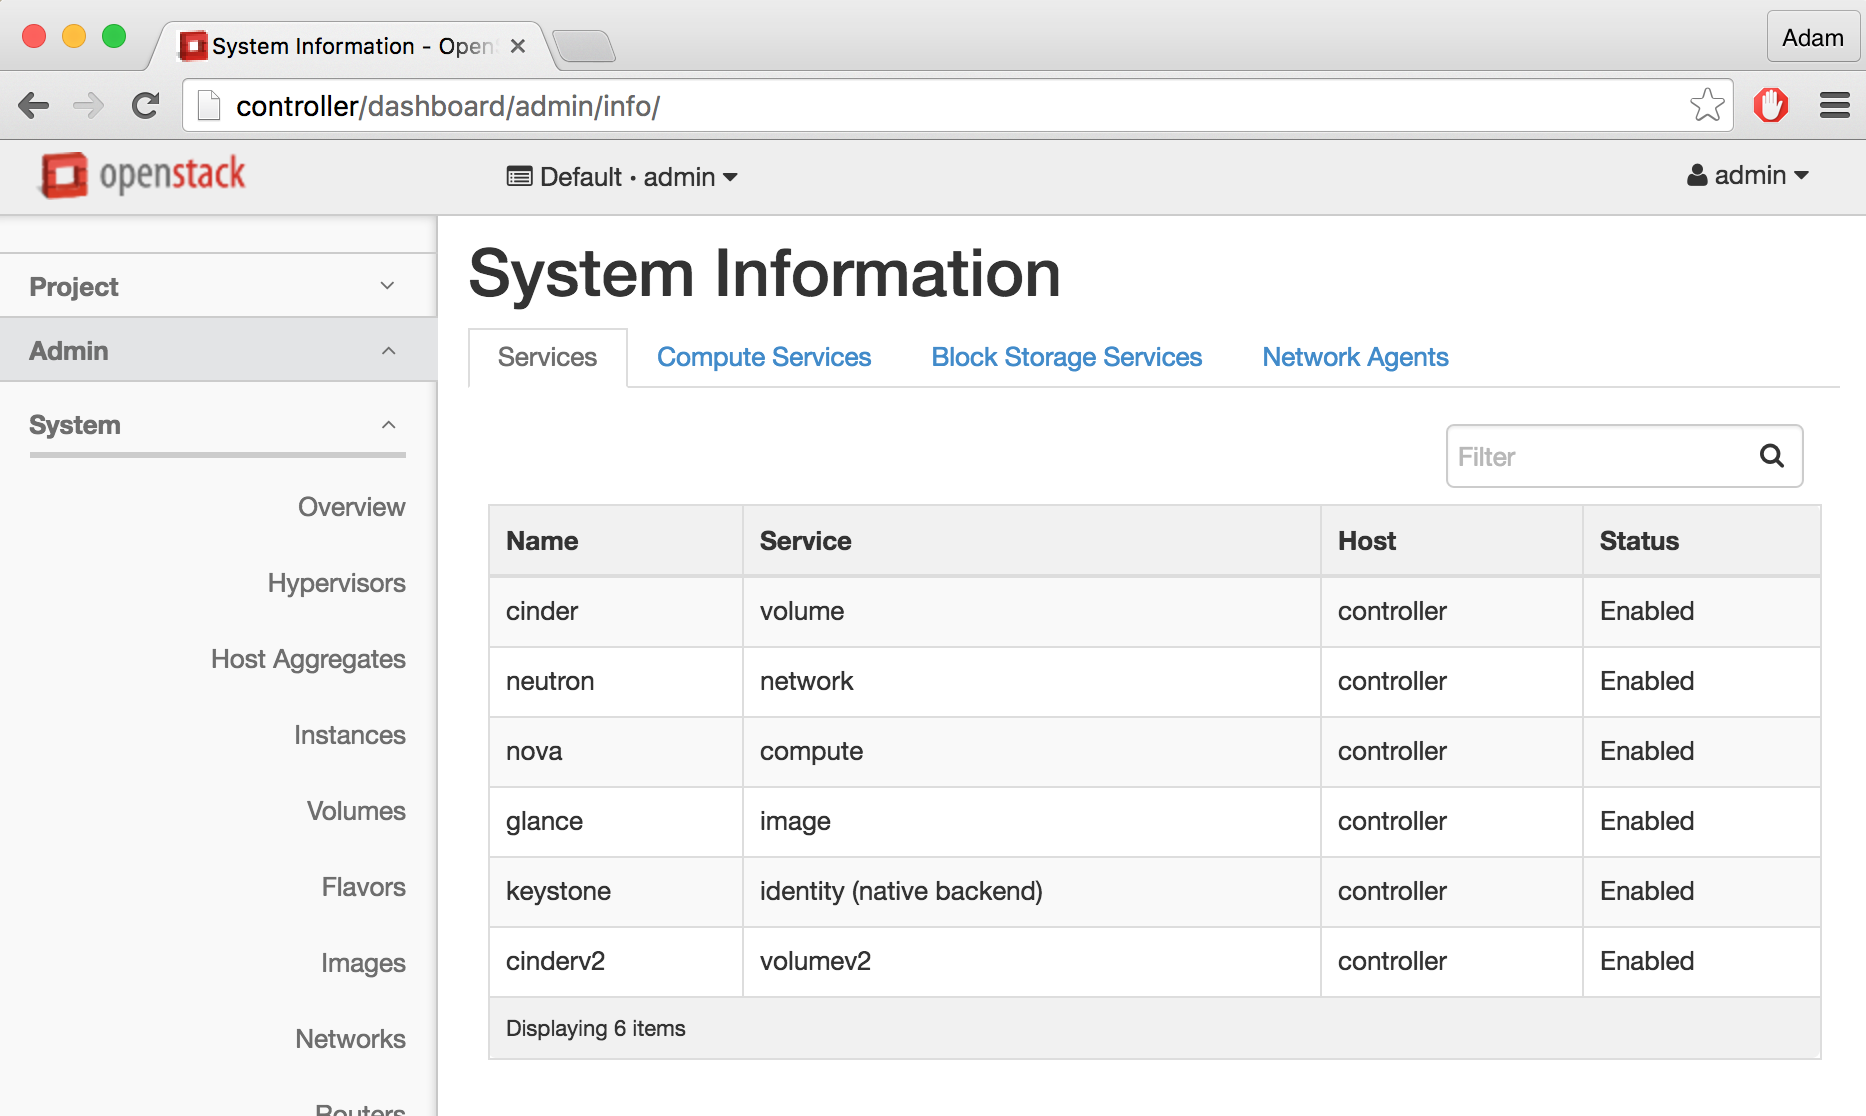
\includegraphics[width=\textwidth]{fig/screenshot_services.png}
  \caption{The OpenStack Dashboard shows the OpenStack services running}
  \label{fig:screenshot_services}
\end{figure}


\begin{figure}[!h]
  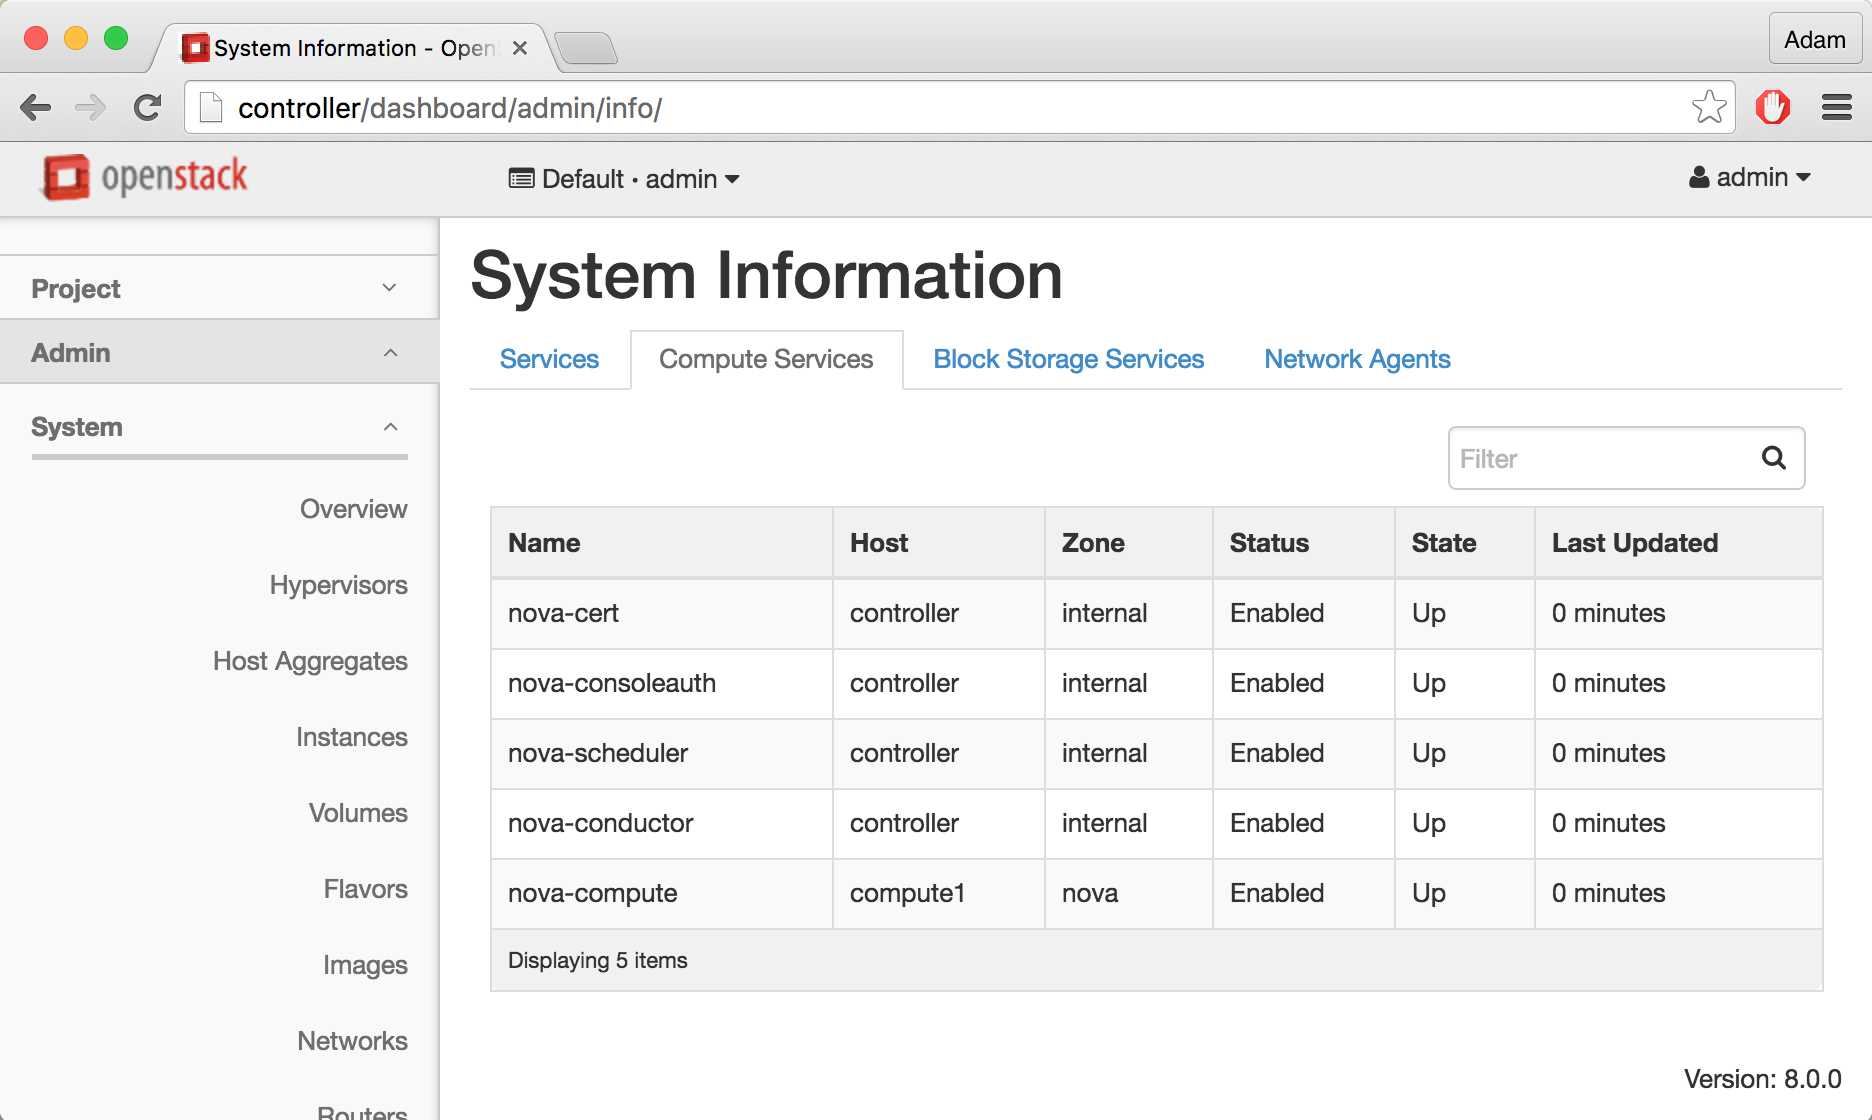
\includegraphics[width=\textwidth]{fig/screenshot_compute.png}
  \caption{The OpenStack Dashboard shows the compute services running}
  \label{fig:screenshot_compute}
\end{figure}


\begin{figure}[!h]
  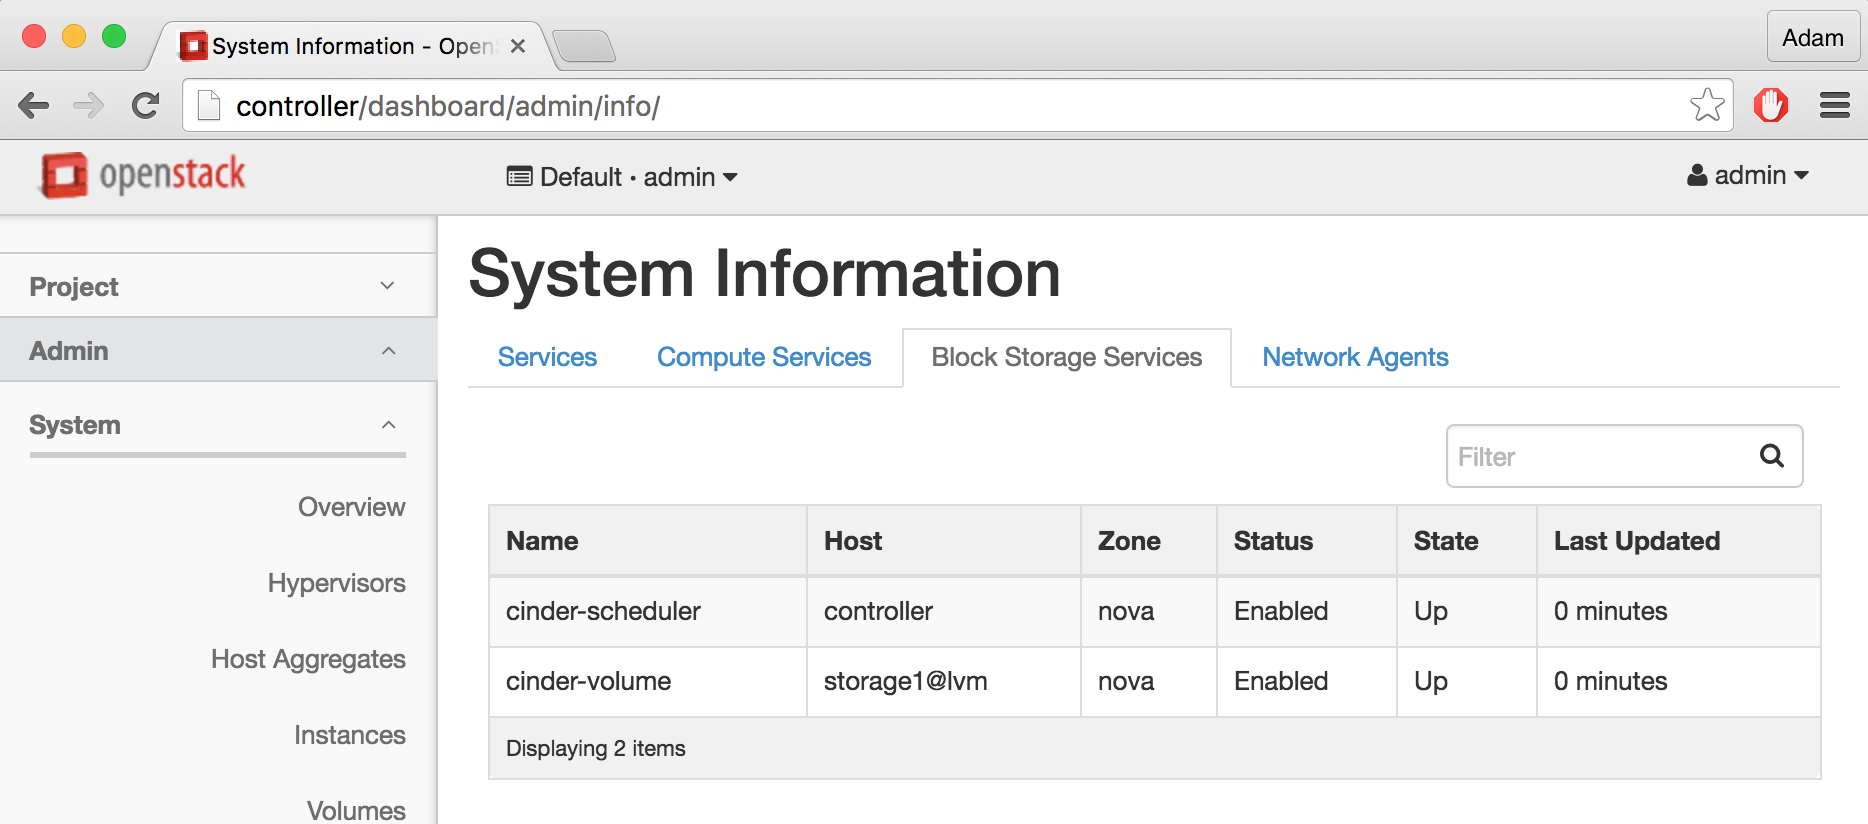
\includegraphics[width=\textwidth]{fig/screenshot_storage.png}
  \caption{The OpenStack Dashboard shows the block storage services running}
  \label{fig:screenshot_storage}
\end{figure}


\begin{figure}[!h]
  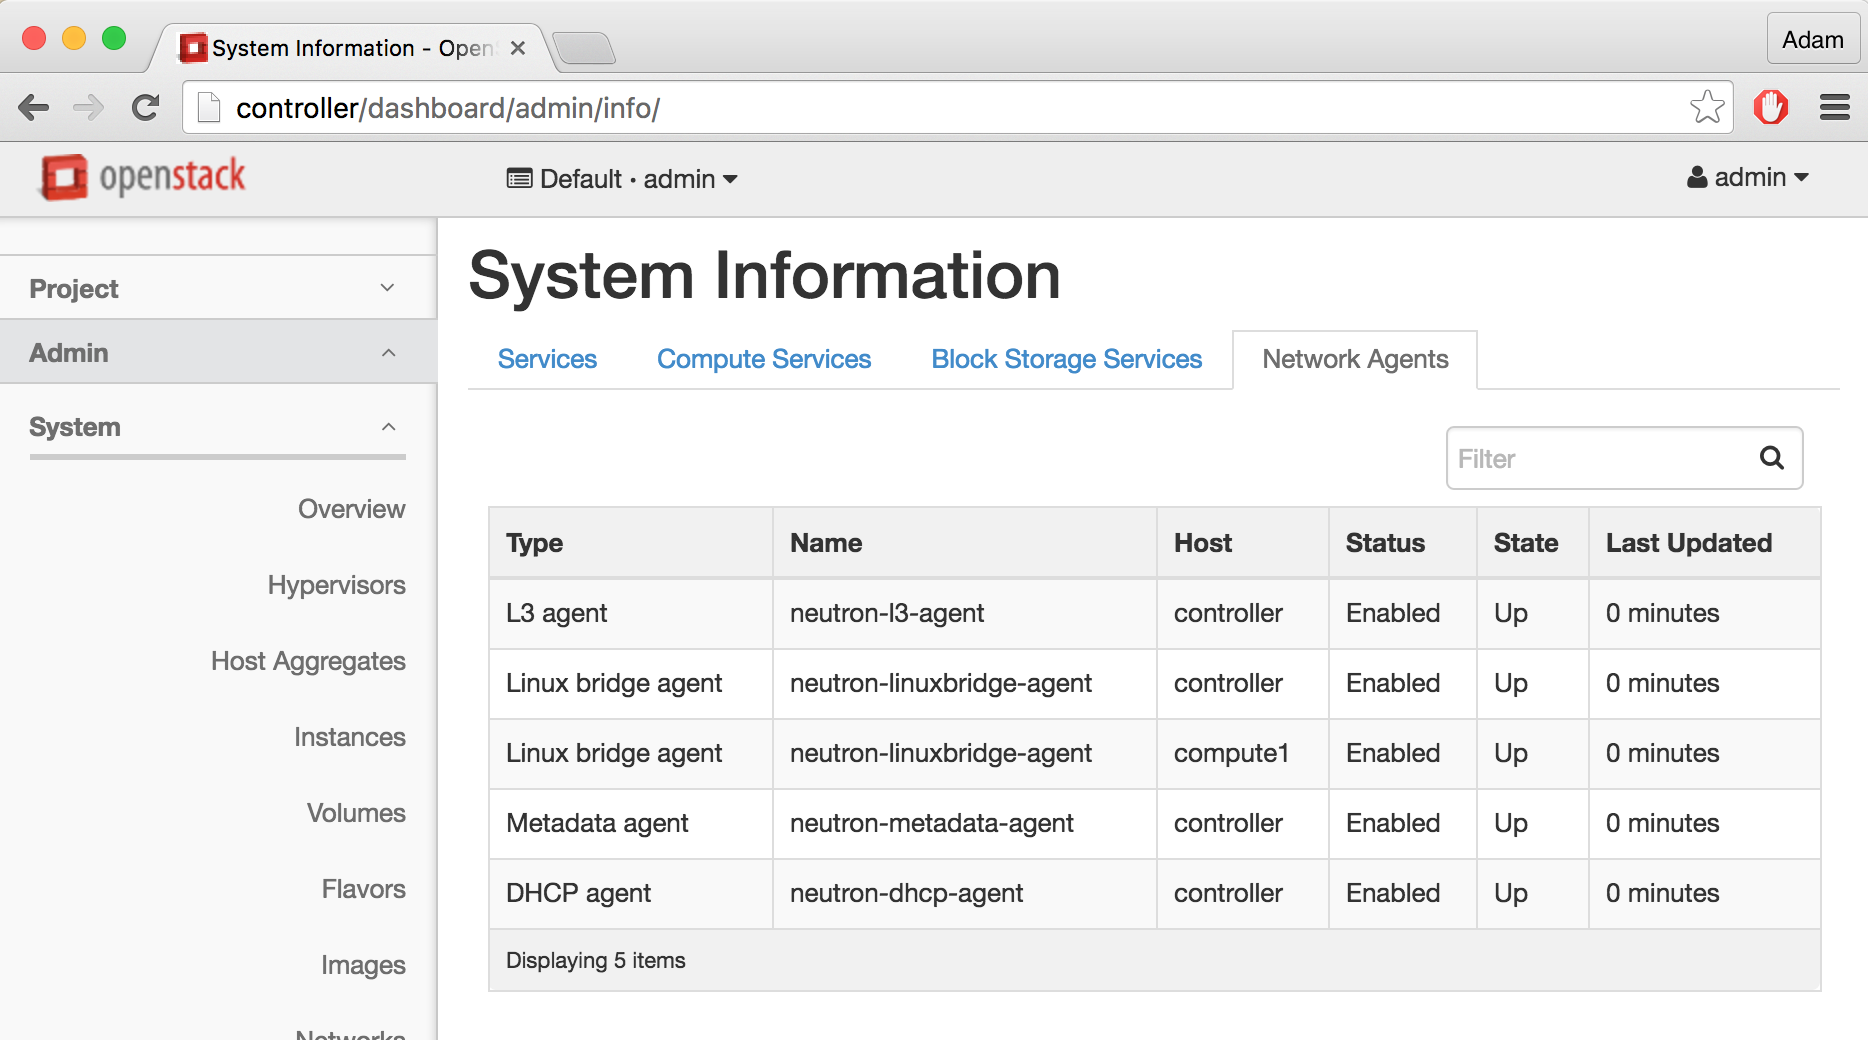
\includegraphics[width=\textwidth]{fig/screenshot_network.png}
  \caption{The OpenStack Dashboard shows the network agents running}
  \label{fig:screenshot_network}
\end{figure}


\subsubsection{Testing the Functionality}

To test the deployment functionality, I have created six virtual machines, two tenant networks, one router, and one provider network. The picture \ref{fig:screenshot} is a screenshot showing the whole environment running in the OpenStadk Dashboard.


\begin{figure}[!h]
  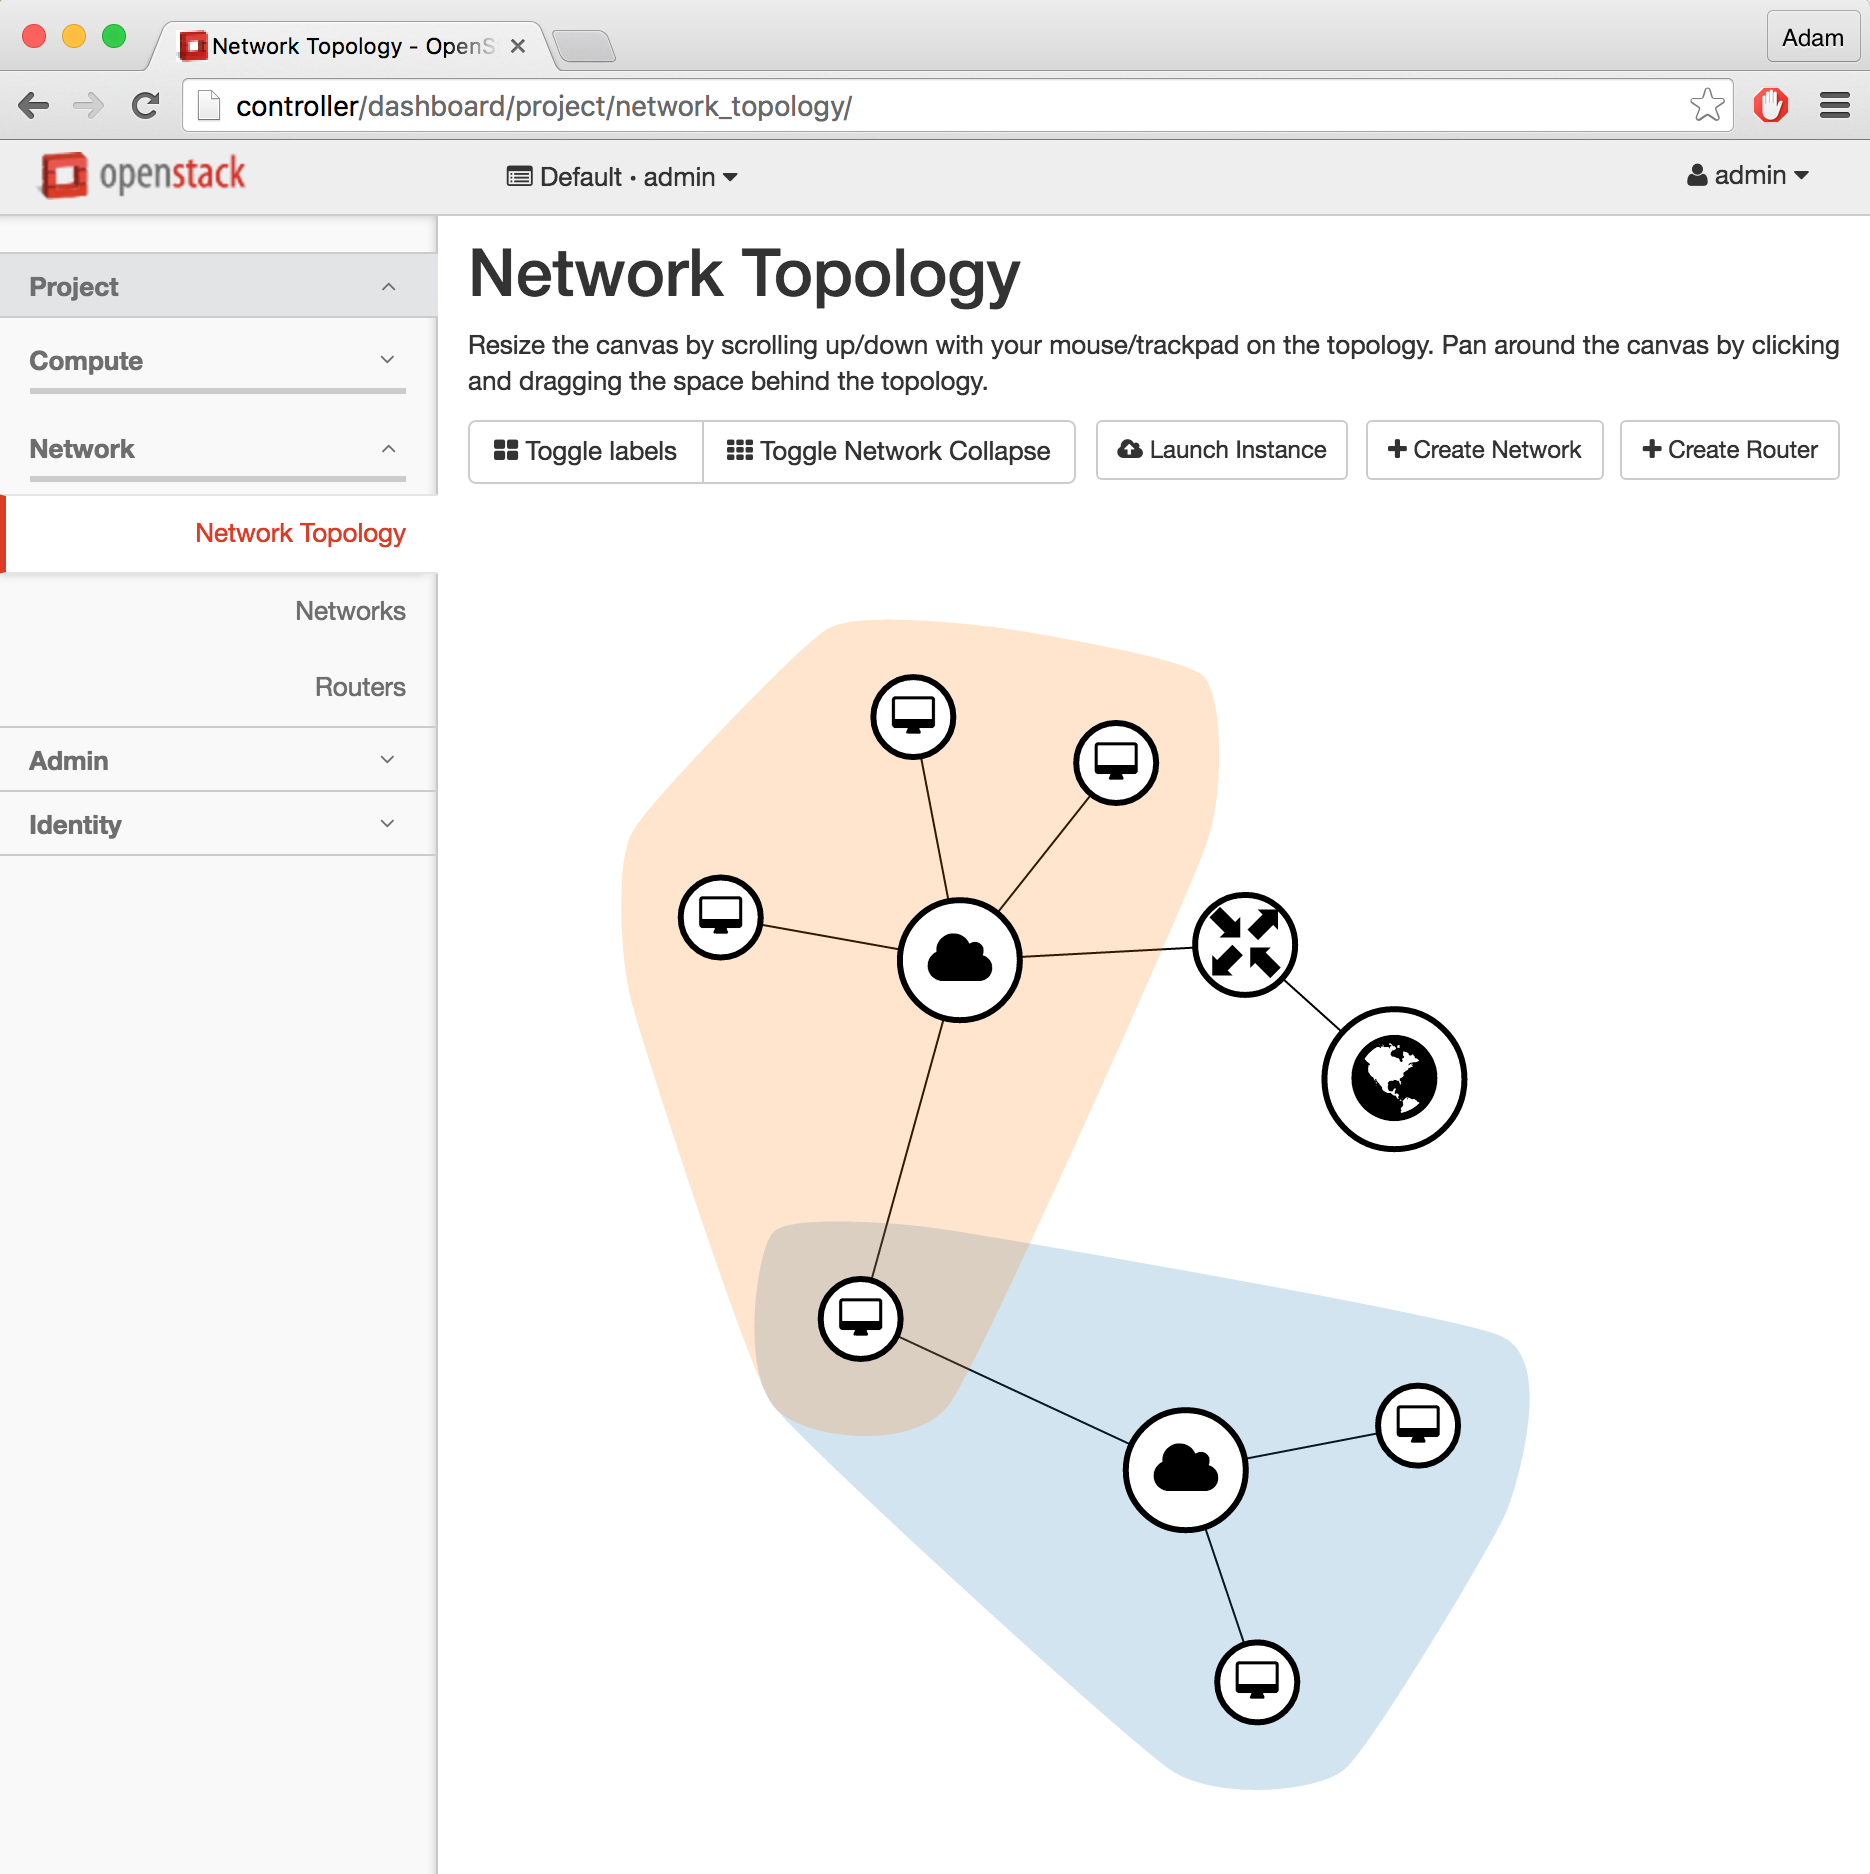
\includegraphics[width=\textwidth]{fig/screenshot.png}
  \caption{The OpenStack Dashboard shows the testing environment}
  \label{fig:screenshot}
\end{figure}

\chapter{Conclusion}
\label{ch:conclusion}
In this Thesis, I have designed simple OpenStack architecture able to run virtual machines, create tenant networks using software-defined networking (SDN), and use persistent storage. This runs in a multi-tenant environment and is managed by a web interface.

I have also designed and implemented an Ansible playbook which can automatically deploy the architecture on multiple physical hosts. This playbook has been designed to be easy to use to deploy the reference architecture, and, at the same time, to be reusable with modifications for deploying different production environments. The reusability is also simplified by using Ansible roles. There is a separate role for each functionality and they can be deployed on separate hosts.

In comparison to Packstack, it offers more flexibility in terms of architecture changes. This is because I have not used the high level of abstraction Packstack uses. This means that customising the playbook will require much deeper knowledge of the OpenStack cloud compared to using Packstack. While this is an advantage for experienced OpenStack administrators, it can be also disadvantage for beginners.

Compared to the official OpenStack-Ansible project, the playbook created in this thesis installs the OpenStack cloud using RPM packages that can be signed and certified before use.

\section{Future Development}

Some roles will be offered to the Fedora Infrastructure team\footnote{https://fedoraproject.org/wiki/Infrastructure} for their own OpenStack infrastructure which is currently installed by Packstack and customized by Ansible. It might require further development and changes to match their architecture, and it will also require extensive testing before using in production.


  % Pouzita literatura
  % ----------------------------------------------
\ifslovak
  \makeatletter
  \def\@openbib@code{\addcontentsline{toc}{chapter}{Literatúra}}
  \makeatother
  \bibliographystyle{czechiso}
\else
  \ifczech
    \makeatletter
    \def\@openbib@code{\addcontentsline{toc}{chapter}{Literatura}}
    \makeatother
    \bibliographystyle{czechiso}
  \else
    \makeatletter
    \def\@openbib@code{\addcontentsline{toc}{chapter}{Bibliography}}
    \makeatother
    \bibliographystyle{plain}
  %  \bibliographystyle{alpha}
  \fi
\fi
  \begin{flushleft}
  \bibliography{literatura} % viz. literatura.bib
  \end{flushleft}

  % Prilohy
  % ---------------------------------------------
  \appendix
\ifczech
  \renewcommand{\appendixpagename}{Přílohy}
  \renewcommand{\appendixtocname}{Přílohy}
  \renewcommand{\appendixname}{Příloha}
\fi
\ifslovak
  \renewcommand{\appendixpagename}{Prílohy}
  \renewcommand{\appendixtocname}{Prílohy}
  \renewcommand{\appendixname}{Príloha}
\fi
  \appendixpage

\ifslovak
  \section*{Zoznam príloh}
  \addcontentsline{toc}{section}{Zoznam príloh}
\else
  \ifczech
    \section*{Seznam příloh}
    \addcontentsline{toc}{section}{Seznam příloh}
  \else
    \section*{List of Appendices}
    \addcontentsline{toc}{section}{List of Appendices}
  \fi
\fi
  \startcontents[chapters]
  \printcontents[chapters]{l}{0}{\setcounter{tocdepth}{2}}
  %\chapter{Obsah CD}
%\chapter{Manual}
%\chapter{Konfigrační soubor}
%\chapter{RelaxNG Schéma konfiguračního soboru}
%\chapter{Plakat}

 % viz. prilohy.tex
\end{document}
